% Autor: Manuel Lippert
% Physikalisches Praktikum

% Main-Datei für die Auswertung in TeX

% Struktur:
% Jedes Kapitel hat einen Input-File. Um Merge-Konflikte zu verhindern wird angeraten für jede 
% Datei eine eigene Tex Datei zu machen und sie im jeweiligen Kapitel zu importieren. Die in
% Input-Struktur dient zur besseren Übersicht und für mögliche Ordner, welche hier vorhanden sind. Die Zahlen vor den 
% Ordner dient zur Ordnung der einzelnen tex-Files nach Kapiteln


% Packages
\documentclass[paper=a4,bibliography=totoc,BCOR=10mm,twoside,numbers=noenddot,fontsize=11pt]{scrreprt}
\usepackage[ngerman]{babel}
\usepackage[T1]{fontenc}
\usepackage[latin1, utf8]{inputenc} %ä, ö, ü inbegriffen
\usepackage[babel,german=quotes]{csquotes} %For Quotes
\usepackage{lmodern}
\usepackage{graphicx}
\usepackage{nicefrac}
\usepackage{fancyvrb}
\usepackage{amsmath,amssymb,amstext}
\usepackage{siunitx}
\usepackage{url}
\usepackage{natbib}
\usepackage{microtype}
\usepackage[format=plain]{caption}
\usepackage{physics}
\usepackage{titleref} 

% Zusätzliche Packages
\usepackage{geometry} % Verändert Seitengeometrie
\usepackage{anyfontsize} % Alle Schriftgrößen möglich machen
\usepackage[table]{xcolor} % Farbliche Gestaltung Tabellen
\usepackage{ifthen} % Für kompliziertere tex-Files
\usepackage[absolute,overlay]{textpos} %Textboxen
\usepackage{amsfonts} % Schriftarten
\usepackage{xstring} % Stringoperationen
\usepackage{tikz} % Zeichnungen
\usepackage{pdfpages} % Import von pdfs (Protokolle)
\usepackage{hyperref} % Verlinkungen im Dokument

% Abschnittseinrückung und -abstand
% Die folgenden Zeilen sollen möglichst nicht verändert werden
\parindent 0.0cm
\parskip 0.8ex plus 0.5ex minus 0.5ex

% Anzahl und Größe von Gleitobjekten
% maximal 2 Objekte oben und unten
% erlaubt auch größere Bilder, welche die ganze Seite benötigen
% Die folgenden Zeilen sollen möglichst nicht verändert werden
\setcounter{bottomnumber}{2}
\setcounter{topnumber}{2}
\renewcommand{\bottomfraction}{1.}
\renewcommand{\topfraction}{1.}
\renewcommand{\textfraction}{0.}

%\sc und \bc veraltet. Daher: (20.09.2018)
\DeclareOldFontCommand{\sc}{\normalfont\scshape}{\@nomath\sc}
\DeclareOldFontCommand{\bf}{\normalfont\scshape}{\textbf}

% Verschiedenes
\pagestyle{headings}          % Der Seitenstil sollte möglichst nicht verändert werden
\graphicspath{{./Bilder/}}    % Der Pfad für die Abbildungen Abbildungen wird gesetzt
\VerbatimFootnotes            % \verb etc. auch in \footnotes mφglich

% Funktionen
\newcommand\tab[1][1cm]{\hspace*{#1}}
\newcommand{\vect}[1]{\boldsymbol{\mathbf{#1}}}
\newcolumntype{g}{>{\columncolor[rgb]{ .741,  .843,  .933}}l}

\begin{document}

    \nonfrenchspacing

    % 0. Kapitel Cover
    % 0. Cover

% Hier sind nur die Variablen und der Abschnitt Informationen (unten) zu bearbeiten der REst läuft automatisch ab (z.b Farbenänderung)

% Noch abänderbar nur ein Vorschlag
\newgeometry{top=30mm, bottom=20mm, inner=20mm, outer=20mm}
\thispagestyle{empty}

% Colors (Notability Colors)
\definecolor{Notablue}{HTML}{3498DB}		
\definecolor{Notared}{HTML}{CF366C}			
\definecolor{Notagreen}{HTML}{19B092}		
\definecolor{Notaorange}{HTML}{FA9D00}		
\definecolor{Notagrey}{HTML}{969696}		
\definecolor{Notalavendel}{HTML}{9DBBD8}	

% Boolean by default false. Für Absatz in der Überschrift
\newboolean{twoRows}
\newboolean{symbol}

% Funktions
\makeatletter
   \def\vhrulefill#1{\leavevmode\leaders\hrule\@height#1\hfill \kern\z@}
\makeatother
\newcommand*\ruleline[1]{\par\noindent\raisebox{.8ex}{\makebox[\linewidth]{\vhrulefill{\linethickness}\hspace{1ex}\raisebox{-.8ex}{#1}\hspace{1ex}\vhrulefill{\linethickness}}}}

% Variables
\def\schriftgrosse{30}
\def\linethickness{1,5pt}

\def\farbe{black}
\def\fach{PPD}
\def\name{Manuel Lippert - Paul Schwanitz}
\def\titel{Dünnfilmprozessierungstechniken \\[0,5cm] und \\[0,5cm] Filmhomogenität} % Absatz mit \\[0,5cm]
\def\bottom{SS2023}
\def\datum{28.03.2023}
\def\platz{Chemie- und Charakterisierungslaber der Gruppe Herzig}
\def\betreuer{Fabian Eller}

% Für Fortgeschrittenen Praktikum siehe unten
\def\teilnehmerm{Manuel Lippert}
\def\emailm{Manuel.Lippert@uni-bayreuth.de}
\def\teilnehmerp{Paul Schwanitz}
\def\emailp{Paul.Schwanitz@uni-bayreuth.de}

% Für Grundpraktikum siehe unten
\def\auswertp{Teilnehmer1}
\def\messp{Teilnehmer2}
\def\protop{Teilnehmer3}

\def\groupnr{1}

\begin{titlepage}
			
	\centering
	{\LARGE \sffamily {\textbf{\bottom}\par}}
	\vspace{2,5cm}
    {\fontsize{30}{0}\sffamily\ruleline{\textcolor{\farbe}{\textbf{\fach}}}\par}
    \vspace{6cm}
	{\Large\sffamily \ruleline{\name}\par}
		
	\IfSubStr {\titel} {\\[0,5cm]} {\setboolean{twoRows}{true}} {\setboolean{twoRows}{false}}
	
	\ifthenelse{\boolean{twoRows}}
		{
			\begin{textblock*}{21cm}(0cm,8cm) % {block width} (coords), centered		
				{\fontsize{\schriftgrosse}{0}\sffamily\textcolor{\farbe}{\textbf{\titel}}\par}
			\end{textblock*}
		}
		{
			\begin{textblock*}{21cm}(0cm,9cm) % {block width} (coords), centered		
				{\fontsize{\schriftgrosse}{0}\sffamily\textcolor{\farbe}{\textbf{\titel}}\par}
			\end{textblock*} 
		}
	
	% Choose Logo
	\ifthenelse {\equal{\farbe}{Notared}} {\def\logo{Bilder/Logo/UniBTNotared}}
		{\ifthenelse {\equal{\farbe}{Notagreen}} {\def\logo{Bilder/Logo/UniBTNotagreen}}
			{\ifthenelse {\equal{\farbe}{Notablue}} {\def\logo{Bilder/Logo/UniBTNotablue}}
				{\ifthenelse {\equal{\farbe}{Notaorange}} {\def\logo{Bilder/Logo/UniBTNotaorange}}
					{\ifthenelse {\equal{\farbe}{Notagrey}} {\def\logo{Bilder/Logo/UniBTNotagrey}}
						{\ifthenelse {\equal{\farbe}{Notalavendel}} {\def\logo{Bilder/Logo/UniBTNotalavendel}}	
							{\ifthenelse {\equal{\farbe}{black}} {\def\logo{Bilder/Logo/UniBT}}	
								{\def\logo{noLogo}}
							}
						}
					}
				}
			}
		}	

	\IfSubStr{\logo}{noLogo}{\setboolean{symbol}{false}}{\setboolean{symbol}{true}}
	
	% Gruppe
	\vspace{10cm}
	{\large\sffamily{Gruppe \groupnr}}
	
	%Logo
	\vfill

	\ifthenelse{\boolean{symbol}}
		{
			\begin{figure}[h]
			\begin{center}
				
				\includegraphics[width=2cm]{\logo}
				
			\end{center}
			\end{figure}
		}
	
\end{titlepage}

\restoregeometry

% Information
\chapter*{Informationen}
\label{chap:info}

\begin{tabular}{l l}

	{\textbf{Versuchstag}} \hspace{1cm} & \hspace{1cm} {\datum}\\[0,2cm]
	{\textbf{Versuchsplatz}} \hspace{1cm} & \hspace{1cm} {\platz}\\[0,2cm]
	{\textbf{Betreuer}} \hspace{1cm} & \hspace{1cm} {\betreuer}\\[1,2cm]
	{\textbf{Gruppen Nr.}} \hspace{1cm} & \hspace{1cm} {\groupnr}\\[0.2cm]
	% Für Fortgeschittenenen Praktikum
	{\textbf{Teilnehmer}} \hspace{1cm} & \hspace{1cm} {\teilnehmerm~(\emailm)}\\[0.2cm]
						  \hspace{1cm} & \hspace{1cm} {\teilnehmerp~(\emailp)}\\[0.2cm]
	% Für Grundpraktikum
	%{\textbf{Auswertperson}} \hspace{1cm} & \hspace{1cm} {\auswertp}\\[0.2cm]
	%{\textbf{Messperson}} \hspace{1cm} & \hspace{1cm} {\messp}\\[0.2cm]
	%{\textbf{Protokollperson}} \hspace{1cm} & \hspace{1cm} {\protop}\\[0.2cm]

\end{tabular}

    \thispagestyle{empty}
    \cleardoublepage
    \tableofcontents
    \cleardoublepage

    % 1. Kapitel Einleitung
    % 1. Einleitung

\chapter{Einleitung}
\label{chap:einleitung}

Dieser Versuch nutzt Interferenzeffekte verusacht von einer Halogen-Deuterium-Lampe (Weißlicht), um optische Eigenschaften von lichtdurchlässigen Materialien zu untersuchen. Die Dicke dieser sog. dünnen Filme reicht dabei von einigen Nano- bis Mikrometern und können durch Reflexion als auch durch Transmission gemessen werden.

Mit diesen Messmethoden lassen sich der Brechungsindex, die Schichtdicke des Films und die Oberflächenbeschaffenheit (Homogenität) bestimmen. Die vergleichsweise simple, nicht destruktive Art der Messung und der geringe Aufwand der Probenpräparation machen diese Messmethode für Laboranwendungen besonders attraktiv und auch für diesen Praktikums Versuch.

Wir betrachten hierbei mehrere Proben mit unterschiedlichen Konzentrationen an Polystyrol und Chlorbenzol aufgebracht auf Glas (Substart) via Spincoating und Vergleichen die jeweilgen Messmethoden.

    % 2.Kapitel Fragen zur Vorbereitung
    % 2. Fragen zur Vorbereitung

\chapter{Fragen zur Vorbereitung}
\label{chap:fvz}

% Text

% Input der Teilaufgaben je nach Produktion der Nebendateien ohne Ordner
% Teilaufgabe 1

\section{Rauschquellen}

\paragraph*{Quantenrauschen}
Aufgrund der Quantisierung des Lichtes (in Photonen) ist es aus statistischen Gründen unmöglich, dass die Intensität der Lichtes absolut konstant ist. Es gilt folgender Zusammenhang für das mittlere Quadrat des Rauschstromes:
\begin{gather}
    i^2_Q = 2ei_{Ph}\Delta \nu = \frac{2e^2\beta_D}{hc}\lambda P \Delta \nu
\end{gather}
wobei\\
\begin{tabular}{rl}
    $e$: & Elementarladung \\
    $i_{Ph}$: & Photonenstrom des Detektors\\
    $\Delta \nu$: & Detektionsbandbreite\\
    $\beta_D$: & Quantenausbeute (Nachweiswahrscheinlichkeit) des Detektors\\
    $\lambda$: & Wellenlänge\\
    $P$: & Lichtleistung\\
    $h$: & Planksches Wirkungsquantum\\
    $c$: & Lichtgeschwindigkeit
\end{tabular}\\
Es ist deutlich zu sehen, dass das Quantenrauschen mit der Quantenausbeute, der Wellenlänge, der Lichtleistung und der Detektionsbandbreite ansteigt.

\paragraph*{Thermisches Rauschen der Photodiode}
Dieses Rauschen ensteht durch die thermische Bewegung der Elektronen in der Photodiode. Die thermische Rauschleistung ergibt sich folgendermaßen:
\begin{gather}
    P_T = 4 k_B T \Delta \nu
\end{gather}
wobei $k_B$ der Boltzmannfaktor, $T$ die absolute Temperatur ist und $\Delta \nu$ die Detektionsbandbreite. Somit ist auch klar ersichtlich, dass dieses Rauschen mit der Temperatur und Detektionsbandbreite zunimmt.


\paragraph*{Technisches Laserrauschen}
Dieses Rauschen tritt Aufgrund der Technischen eigenheiten des Lasers auf. Beispielsweise kann dieses Rauschen durch Schwingungen der Laserspiegel zueinander oder Instabilitäten in der Gasentladung, bei Gaslasern, verursacht werden. Eine Besonderheit dieses Rauschens ist es, dass es nicht weiß ist, sondern es vor allem bei niedrigen Frequenzen auftritt. Oberhalb einiger MHz ist es dann vernachlässigbar. 

% Teilaufgabe X

\section{Vergleich thermisches Rauschen und Quantenrauschen}
\label{sec:rauschen}

Im Folgenden soll die Leistung (in dBm) de thermischen Rauschens und des Quantenrauschens für folgenden Fall berechnet werden:

$P = 0,1$ mW, $T = 293$ K, $R = 50\, \Omega$, $\beta_D = 0,3$ und $\Delta \nu = 10$ kHz.

Für die Leisungsschwankung, welch durch Quantenrauschen verursacht wird, gilt:
\begin{align}
    \Delta P_\mathrm{Q} &= i^2_\mathrm{Q} \cdot R = \frac{2e^2\beta_\mathrm{D}}{hc}\lambda P \Delta \nu \cdot R \\
    \Delta P_\mathrm{Q} &= \frac{2e^2 \cdot 0,3}{hc} \cdot (632,8 \cdot 10^{-9}) \, \mathrm{m} \cdot (0,1 \cdot 10^{-3})\, \mathrm{W} \cdot (10 \cdot 10^3) \, \mathrm{Hz} \cdot 50 \, \Omega \\
    \Delta P_\mathrm{Q} &= 2,45 \cdot 10^{-15}\,\mathrm{mW} \qquad \Rightarrow \quad \Delta P_\mathrm{Q}^* = -146 \, \mathrm{dBm}
\end{align}

Für das thermische Rauschen gilt:
\begin{gather}
    P_\mathrm{T} = 4 \cdot k_\mathrm{B} \cdot 293\,\text{K} \cdot 10\,\text{kHz} = 1,62 \cdot 10^{-13}\, \text{mW} \qquad \Rightarrow \quad P_\mathrm{T}^* = -128 \, \text{dBm}
\end{gather}

Es ist zu erkennen, dass das Quantenrauschen gegenüber dem thermischen Rauschen zu vernachlässigen ist.
Somit reicht es die Verstärkung und die Verringerung von 6\,dbm \cite{anleitung} auf das thermische Rauschen anzuwenden, um den Rauschpegel zu erhalten:
\begin{gather}
    P_\mathrm{R,Theo}^* = -128 \, \text{dBm} + 55\, \text{dBm} - 6 \, \text{dBm}= -79 \, \text{dBm}
\end{gather}
% Teilaufgabe 3

\section{Dunkelfeldmikroskop in Transmission}
\label{sec:mikroskop}

\subsection{Aufbau und Funktionsweise}
\label{sub:aufbau}

\begin{center}
    \captionsetup{type = figure}
    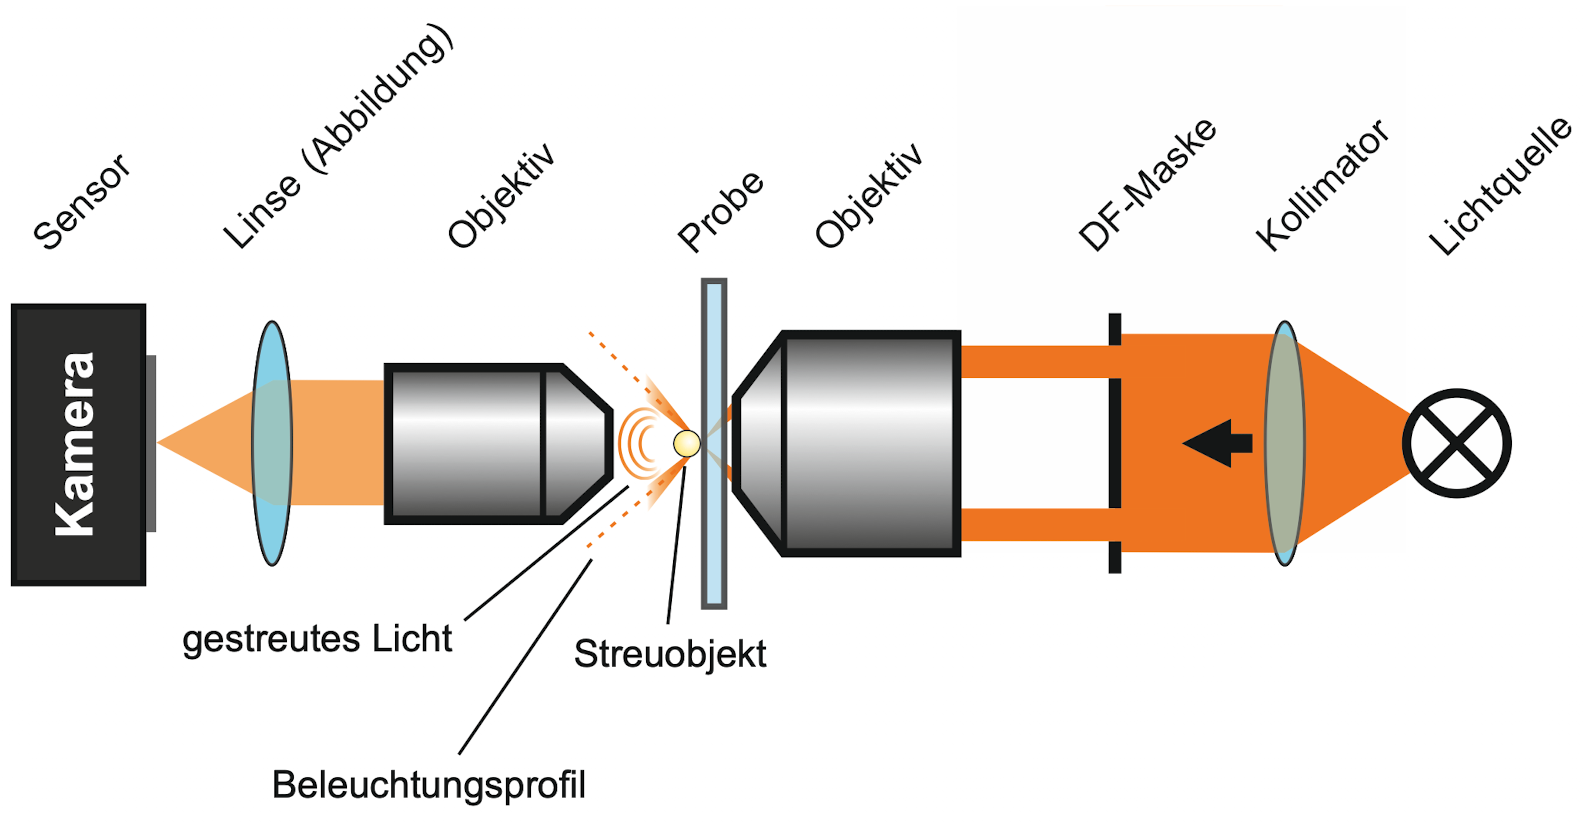
\includegraphics[width = 0.9\textwidth]{Bilder/Aufbau_Dunkelfeld.png}
    \captionof{figure}{Einfacher Aufbau eines Dunkelfeldmikroskops in Transmission. Eine breitbandige Lichtquelle wird mittels einer Optik kollimiert. Eine Maske (DF-Maske) schneidet einen Ring in das Strahlprofil. Der so geformte Strahl wird mittels Objektiv auf die Probe fokussiert. Ein weiteres Objektiv sammelt das von der Probenoberfläche bzw. dem Objekt gestreute Licht auf, wodurch kein direktes Licht der Beleuchtung eingesammelt wird. Das gestreute Licht wird über eine Linse auf den Kamerasensor abgebildet. \cite{Anleitung}}
    \label{fig:aufbau}
\end{center}

Die Dunkelfeldmikroskopie ist eine hintergrundfreie Methode, was bedeutet, dass kein Hintergrundsignal detektiert wird, sondern nur Informationen von dem untersuchten Objekten. In Abb. \ref{fig:aufbau} ist der schematische Aufbau des Dunkelfeldmikroskops in Transimission abgebildet. Auf der rechten Seite steht die Lichtquelle, die mittels einer Linse kollimiert wird. Dahinter befindet sich eine inverse Lochblende (DF-Maske), die lediglich die Ränder des Lichtkegels transmittiert. Mit einem Objektiv relativ hoher numerischer Apertur wird die Probe beleuchtet, wobei auf der anderen Seite der Probe befindet sich ein Objektiv mit geringerer numerischer Apertur. Durch diese besondere Beleuchtung kann kein direktes Erregerlicht in dieses Objektiv fallen, wodurch die Abbildung der Probenoberfläche auf der Kamera dunkel erscheint. Befindet sich jedoch ein Streukörper, zum Beispiel ein Nanopartikel, auf der Probenoberfläche so wird das Erregerlicht daran gestreut, was widerum vom Objektiv aufgesammelt und detektiert werden kann. \cite{Anleitung}

\subsection{Messung von plasmonischen Eigenschaften}
\label{sub:messungEigenschaften}

Das Prinzip der Dunkelfeldmikroskopie beruht darauf, dass Objekte Licht nicht nur absorbieren, sondern auch immer einen Teil des Lichtstrahls ablenken. Die Stärke eines Signals ist bei der Dunkelfeldmikroskopie nicht von der Größe einer Struktur abhängig, sondern davon wie stark das Licht von ihr abgelenkt wird. Eine der Ablenkungsursachen ist die als Tyndall-Effekt bezeichnete Streuung von Licht an kleinen Teilchen, welche beispielsweise auch zu beobachten ist, wenn Licht in einen dunklen Raum fällt und der Staub innerhalb des Lichtstrahls deutlich sichtbar wird. Daher können auch Partikel oder Strukturen nachgewiesen werden, die kleiner sind als die Auflösungsgrenze des jeweiligen Mikroskops. \cite{WikiDunkelfeld}

\subsection{Hintergrundkorrigiertes Dunkelfeldspektrum}
\label{sub:korrigiertesSignal}

In diesem Versuch wird zusätzlich zum hintergrundfreien Streuspektrum der Partikel auch noch das Lampenspektrum der Beleuchtungseinheit, sowie ein Spektrum ohne Beleuchtung aufgenommen. Um ein hintergrundkorrigiertes Dunkelfeldspektrum zu erhalten, wird im folgenden vom Lampenspektrum das Spektrum ohne Beleuchtung abgezogen, was im weiteren als effektives Lampenspektrum bezeichnet wird. Das effektive Lampenspektrum wird wiederum vom Streuspektrum des Partikels abgezogen, wobei hier auch das Spektrum ohne Beleuchtung abgezogen wurde. Nach dieser Argumentation wird klar, dass beide Spektren (Lampenspektrum und Streuspektrum) den gleichen Hintergrund Offset (Spektrum ohne Beleuchtung) teilen. Weshalb vorgeschlagen wird die Korrketur, um den Offset zu vernachlässigen und nur um das Lampenspektrum zu korrigieren. 
% Teilaufgabe 4

\newpage
\section{Stokes Relation}
\label{sec:stokesRelation}

\begin{align}
    t^2 + r^2 = 1 
\end{align}

Die Strokes Relation sagt aus, dass reflektierte und transmittierte Intensität zusammen die Intensität der einfallenden Welle ergeben, sofern keine Absorption durch das Material auftritt.
% Teilaufgabe X

\section{Quecksilberdampflampe als alternative Lichtquelle}

Eine Quecksilberdampflampe eignet sich nicht als Alternative für einen Laser. Wie bereits erwähnt wurde ist für FMS ein monochromatischer Laser, welcher nur in einer Mode schwingt, erforderlich. Diese Anforderungen erfüllt die Quecksilberdampflampe nicht, was zu beträchtlichen Störungen der Messung führt.

Man könnte jedoch Filter benutzen, um die gewünschte Mode herauszufiltern. Dieses Vorgehen ist jedoch mit starken Intensitätseinbusen verbunden, weshalb es auch ungeeignet ist.
% Teilaufgabe X

\section{Phasenmodulation des Laserlichtes}

Das Laserlicht wird in einem elektrooptischen Modulator phasenmoduliert. In diesem befinden sich zwei hintereinander angeordnete LiTaO$_3$-Kristalle. Diese verändern ihren Brechungsindex, für Licht einer bestimmten Polarisation, bei angelegten E-Feld. Mittels Hochfrequenzgenerator wird der Kristall nun angesteuert um die Phase des Laserstrahls zu modulieren.
% Teilaufgabe 7

\newpage
\section{Spektren der verwendeten Lampen dieses Versuches}
\label{sec:spekternLampen}

\begin{enumerate}
	\item Halogenlampe
	\begin{center}
		\captionsetup{type=figure}
		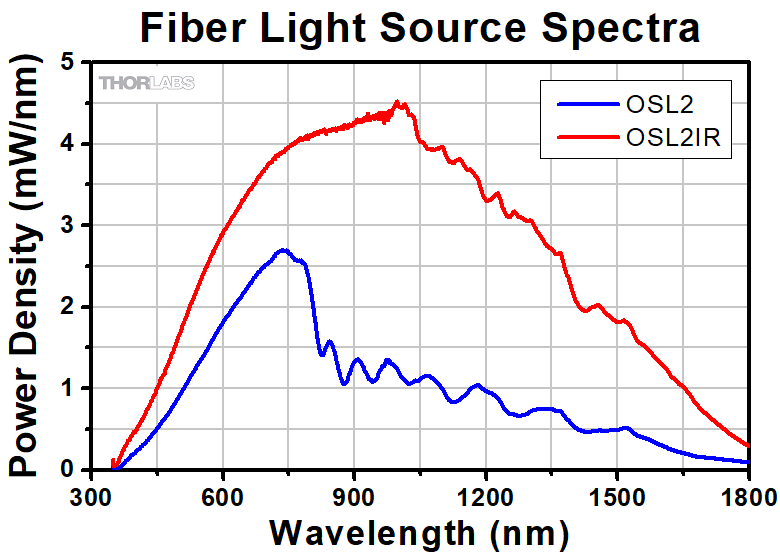
\includegraphics[width=0.75\textwidth]{Spektrum-Halogen.png}
		\captionof{figure}{Spektrum einer Halogenlampe. \cite{halogenlamp}}
		\label{fig:halogen}
	\end{center}
	\item Deuteriumlampe
	\begin{center}
		\captionsetup{type=figure}
		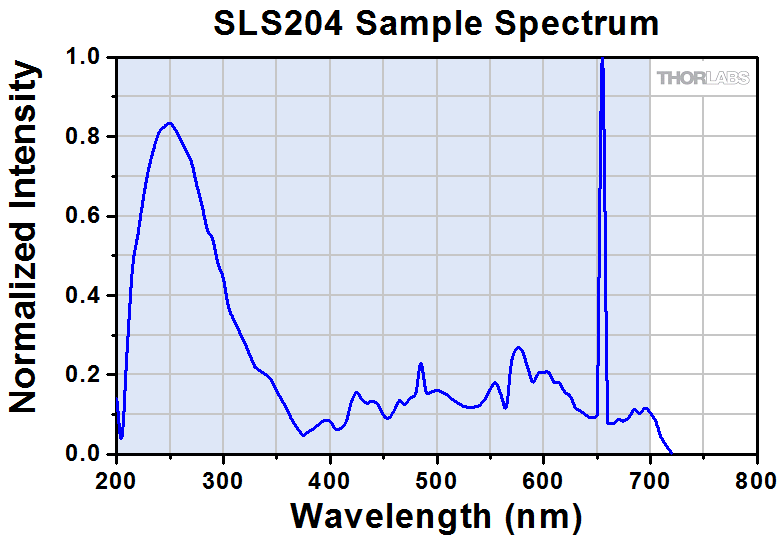
\includegraphics[width=0.75\textwidth]{Spektrum-Deuterium.png}
		\captionof{figure}{Spektrum einer Deuteriumlampe. \cite{deuteriumlamp}}
		\label{fig:deuterium}
	\end{center}
\end{enumerate}

% Teilaufgabe X

\section{Teilaufgabe X}
% Teilaufgabe X

\section{Teilaufgabe X}
% Teilaufgabe X

\section{Zusammenhang zwischen Absorptionskoeffizienten und Brechungsindex}
\label{sec:absorpBrechung}

Der Absorptionskoeffizient $\alpha$ ist proportional zum Imaginärteil des Brechungsindexes $\kappa$.  Dieser Zusammenhang kann mit einer erzwungen elektromagnetischen Schwingung der Form:
\begin{gather}
    m \derivative[2]{x}{t} + b \derivative{x}{t} + Dx = q E_0e^{i\omega t}
    \label{eq:schwingung}
\end{gather}
mit Masse $m$, Ladung $q$, Reibungskonstante $b$ und Rückstellmoment $D$ erklärt werden. Durch Lösen der Gleichung \ref{eq:schwingung} mit dem Ansatz $x=x_0e^{i\omega t}$ und Einsetzen der Lösung in die Gleichung der Polarisation $P = Nqx = \epsilon_0(\epsilon-1)E$ erhält man mit dem Brechungsindex $n$ von nichtferromagnetischen Materialien ($n = \sqrt{\epsilon}$) erhält man:
\begin{gather}
    n^2 = 1 + \frac{Nq^2}{\epsilon_0 m (\omega_0^2 - \omega^2 + i\gamma\omega)}~,
    \label{eq:brechungsindex}
\end{gather}
wobei $\gamma = b/m$ und $\omega_0^2 = D/m$ ist. Der Brechungsindex kann dann in den komplexen Brechungsindex $n(\omega)$ umgeschrieben werden:
\begin{gather}
    n = n' + i\kappa;~~~~ n',\kappa \in \mathbb{R}~.
\end{gather}
Im nächsten Schritt wird eine elektromagnetische Welle der Form:
\begin{gather}
    E = E_0 e^{i(\omega t - Kz)}~\mathrm{mit}~K = 2\pi/\lambda~,
    \label{eq:efeld}
\end{gather}
welche durch das Medium mit dem Brechungsindex $n$ in $z$-Richtung mit der Wellenzahl $K$ läuft. Im Vakuum ist dabei $K = K_0$ und in der Materie $K_\mathrm{M} = nK_0 = n'K_0 -i\kappa K_0$. Setzt man $K_\mathrm{M}$ für $K$ in Gleichung \ref{eq:efeld} ein, erhält man:
\begin{gather}
    E = E_0e^{-K_0\kappa z}e^{i(\omega t -n'K_0z)} = E_0e^{-2\pi \kappa z/ \lambda}e^{iK_0(c_0 t -n'z)}~.
    \label{eq:efeldc}
\end{gather}
Laut Beerschen Absorptionsgesetz ist der Absorptionskoeffizient $\alpha$ für den Intensitätsverlauf gegeben durch:
\begin{gather}
    I = I_0 e^{-\alpha z}~.
    \label{eq:beer}
\end{gather}
Da Intensität proportional zum Quadrat der Amplitude ist, wird Gleichung \ref{eq:efeldc} quadriert und die Exponenten mit denen der Gleichung \ref{eq:beer} verglichen. Der Vergleich ergibt dann:
\begin{gather}
    \boxed{\alpha = 4 \pi \kappa / \lambda = 2K \kappa}~,
\end{gather}
was die zuvor angesprochenen Zusammenhang ergibt. \cite{DemtroederLaser1}
% Teilaufgabe X

\section{Signal vor dem Mischer bei fester Modulationsfrequenz $\omega_\mathrm{m}$}
\label{sec:signalMischer}


% Teilaufgabe X

\section{Herleitungen}
\label{sec:herleitung}

In diesem Kapitel sollen Formel (3.6) und (3.7) aus dem Skript zu diesen Versuch hergeleitet werden. Da das Skript selbst nicht direkt auf den Ursprung der Formeln eingeht, wird diese Herleitung nur kurz mit der Literatur \citenum{FMSpectro} hergeleitet und dem Skript abgearbeitet.

Aus Literatur \citenum{FMSpectro} wird entnommen, dass folgende Relation gilt:
\begin{gather}
    \delta_\mathrm{n} = \alpha_\mathrm{n} \frac{L}{2}~.
    \label{eq:absorp}
\end{gather}
Aus dem Skript entnehmen wir von die Gleichungen (1.1) und (1.2) und setzen sie gleich, was folgende Beziehung ergibt:
\begin{gather}
    \frac{I}{I_0} = e^{-\alpha L} = 10^{-\mathrm{OD}} \Leftrightarrow \alpha = \frac{\ln 10}{L} \mathrm{OD}~.
    \label{eq:absorpkoeff}
\end{gather}
Setzt man nun nur noch Gleichung \ref{eq:absorpkoeff} in Gleichung \ref{eq:absorp} erhält man die gewünschte Beziehung:
\begin{gather}
    \boxed{\delta_\mathrm{n} = \frac{\ln 10}{2} \mathrm{OD}}~.
\end{gather}

Weiterhin wird aus der Literatur \citenum{FMSpectro} entnommen:
\begin{gather}
    \phi_\mathrm{n} = \eta_\mathrm{n} L \left( \frac{\omega_\mathrm{c} + n \omega_\mathrm{m}}{c} \right)~.
    \label{eq:phase}
\end{gather}
Zusammen mit der Überlegungen
\begin{gather}
    c = \lambda f = \lambda \frac{\omega}{2\pi} \Leftrightarrow \frac{2\pi}{\lambda} = \frac{\omega}{c}~\mathrm{mit}~\omega=\omega_\mathrm{c} + n \omega_\mathrm{m}
\end{gather}
muss dann eingesetzt in Gleichung \ref{eq:phase} gelten:
\begin{gather}
    \boxed{\phi_\mathrm{n} = \eta_\mathrm{n} L \left( \frac{2\pi}{\lambda} \right)}~,
\end{gather}
was die gesuchte Gleichung (3.7) aus dem Skript ergibt.
% Teilaufgabe X

\section{Physikalische Eigenschaft der Hyperfeinstruktur von Jod und Brom}
\label{sec:hyperfeinstruktur}

Die Hyperfeinstruktur impliziert die physikalische Eigenschaft, dass die Atomkerne ein magnetisches Moment besitzen. Dabei wird das magnetische Moment in der Quantenmechanik in der Form:
\begin{gather}
    \abs{\vect{I}} = \hbar \sqrt{I\cdot (I+1)}
\end{gather}
beschrieben. \cite{DemtroederKerne} Die Aufspaltung der Hyperfeinstruktur liefern dann zwei Beiträge:
\begin{itemize}
    \item Wechselwirkung des Kernmomentes mit dem Magnetfeld, das von Elektronen am Kernort erzeugt wird (Zeeman-Effekt des Kernmomentes mit dem atomaren Magnetfeld) \cite{DemtroederAtome}
    \item Wechselwirkung des elektronischen magnetischen Moment mit dem vom Kernmoment erzeugten Magnetfeld \cite{DemtroederAtome}
\end{itemize}


% etc.

    % 3.Kapitel Protokoll
    % 3. Protokoll

% Variables
\def\skalierung{0.65}

\chapter{Messprotokoll}
\label{chap:protokoll}

\section{Probenpräparation}
\label{sec:prep}

\subsection{Substratherstellung}
\label{sub:substrat}
Als Substrat werden Glasplätchen verwendet die in passender Länge (~\SI{2,5}{\centi\metre}) und Breite (~ß\SI{1,5}{\centi\metre}) zugeschnitten, welche dann wiederum mit dem Schema \textit{GruppennummerSubstratnummer} (z.Bsp. 13 (Substrat 3) und 111 (Substrat 11)).

\subsection{Stammlösung}
\label{sub:stamm}
Als Stammlösung wird Polystyrol (PS) und Chlorbenzol (CB) verwendet. Diese werden im dem Fläschen \enquote{\textit{PS-CB; \SI{300}{\milli\gram\per\milli\litre}; Gruppe 1}} angerührt. Dabei erhalten wir \SI{297,92}{\milli\gram} PS, was zur Folge hat, dass \SI{0,9931}{\milli\litre} CB zugegeben werden muss, um die gewünschte Konzentration von \SI{300}{\milli\gram\per\milli\litre} zu erhalten.

\subsection{Verdünnung}
\label{sub:verduennung}

Um aus der angesetzte Lösung aus Kapitel \ref{sub:stamm} die gewünschten Konzentration von \SI{1}{\milli\gram\per\milli\litre}, \SI{25}{\milli\gram\per\milli\litre}, \SI{50}{\milli\gram\per\milli\litre}, \SI{100}{\milli\gram\per\milli\litre}, \SI{150}{\milli\gram\per\milli\litre}, \SI{200}{\milli\gram\per\milli\litre} und \SI{250}{\milli\gram\per\milli\litre} zu erhalten, werden folgende Formeln verwendet:
\begin{gather}
	V_0 = V_S + V_{CB}\\
	\boxed{V_{CB} = V_0 \cdot \left( 1 - \frac{c_0}{c_S} \right)}\\
	\Rightarrow \boxed{V_S = V_0 \cdot \frac{c_0}{c_S}}~,
	\label{eq:vol}
\end{gather}
wobei $V_{CB}$ das Volumen von Chlorbenzol, $V_S$ das Volumen der Stammlösung mit der Konzentration $c_S$ und $V_0$ das Endvolumen der verdünnten Lösung mit der gewünschten Konzentration $c_0$ ist. Das Endvolumen $V_0$ wird hierbei frei gewählt. Von \SI{25}{\milli\gram\per\milli\litre} bis \SI{250}{\milli\gram\per\milli\litre} wird die Stammlösung zum verdünnen verwendet, während für die Konzentration \SI{1}{\milli\gram\per\milli\litre} die Konzentration \SI{25}{\milli\gram\per\milli\litre} als Stammfunktion verdünnt wird. Für die Werte zur Verdünnung siehe Tabelle \ref{tab:verduennung}.

\subsection{Spincoating}
\label{sub:spin}

Beim Spincoating wird die verdünnten Konzentrationen aus Kapitel \ref{sub:verduennung} auf die Substrate aus Kapitel \ref{sub:substrat} verteilt. Dabei wird nur die \textbf{Serie 2} (alle Konzentrationen mit 1000\,rpm bei \SI{90}{\sec}) aus der Versuchsanleitung gemacht. Dies hat zur Folge, dass Auswertung (6.2) aus der Versuchsanleitung wegfällt. Die verwendeten Substrate für die jeweilige Konzentrationen können in \ref{tab:verduennung} nachgelesen werden. Als Referenzsubstrate dienen die Proben \textit{19}, \textit{11}, \textit{111} und \textit{112} verwendet.

\begin{center}
	\captionsetup{type=table}	
	\begin{tabular}{r | r | r r | l}
		$c_0$/\si{\milli\gram\per\milli\litre} & $V_0$/\si{\micro\litre}  & $V_S$/\si{\micro\litre} & $V_{CB}$/\si{\micro\litre} & Substrat \\[0,1cm]
		\hline
		300  &  $933 - V_{S;250-25} = 373$  &  373  &    0  &   12 \\
		250  &  					  240   &  200  &   40  &   13 \\
		200  &  					  240   &  160  &   80  &   14 \\
		150  &  					  240   &  120  &  120  &   15 \\
		100  &  					  240   &   80  &  160  &   16 \\
		 50  &  					  240   &   40  &  200  &   17 \\
		 25  &  $240 - V_{S;1}		= 220$  &   20  &  220  &   18 \\
		  1  &  					  500   &   20  &  480  &  110 \\
	\end{tabular}
	\captionof{table}{Werte für die Verdünnung}
	\label{tab:verduennung}
\end{center}

\section{Spektroskopie}
\label{sec:spectroskopie}

Es werden für jede Konzentration eine Reflexions- und Transmissionsmessung gemacht. Dabei wird eine Halogen-Deuterium-Lampe der Firma \textit{OceanOptics} mit der Inventarnummer 107628 verwendet [Abb. \ref{fig:lampe}].
\begin{center}
	\captionsetup{type=figure}
	\begin{tabular}{c c}
		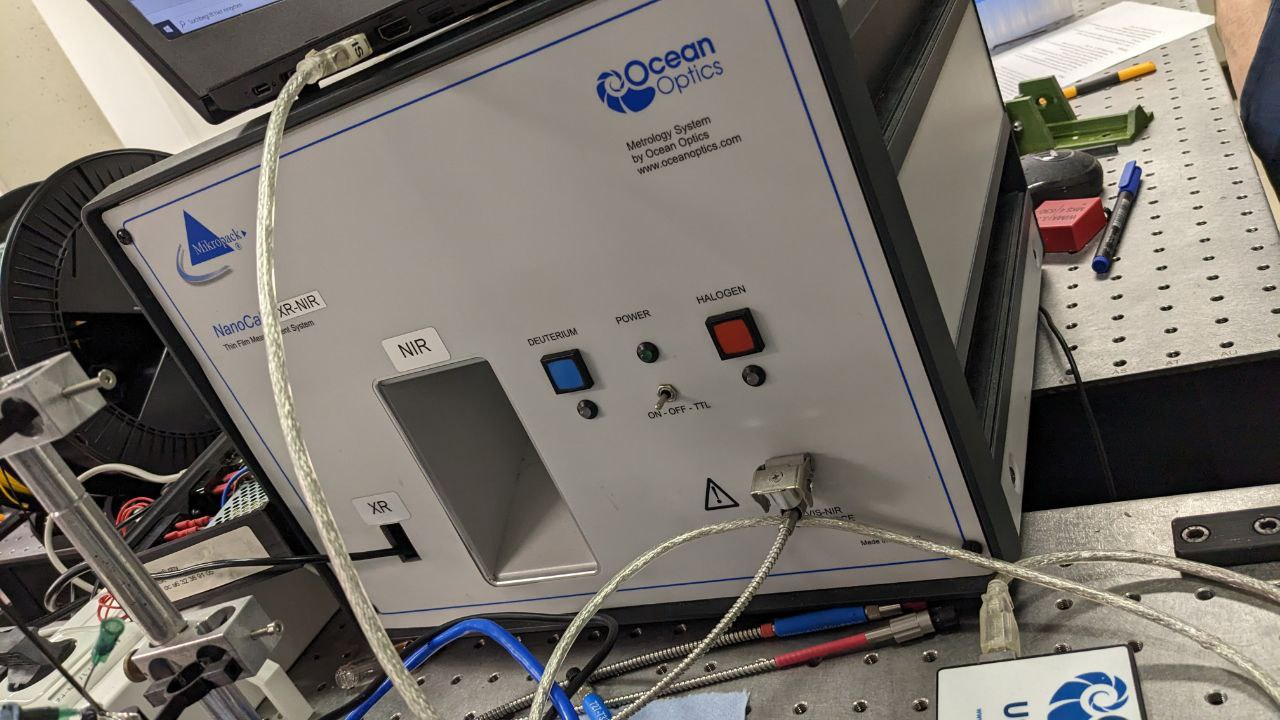
\includegraphics[scale = 0.15]{Lichtquelle-vorne.jpg} & 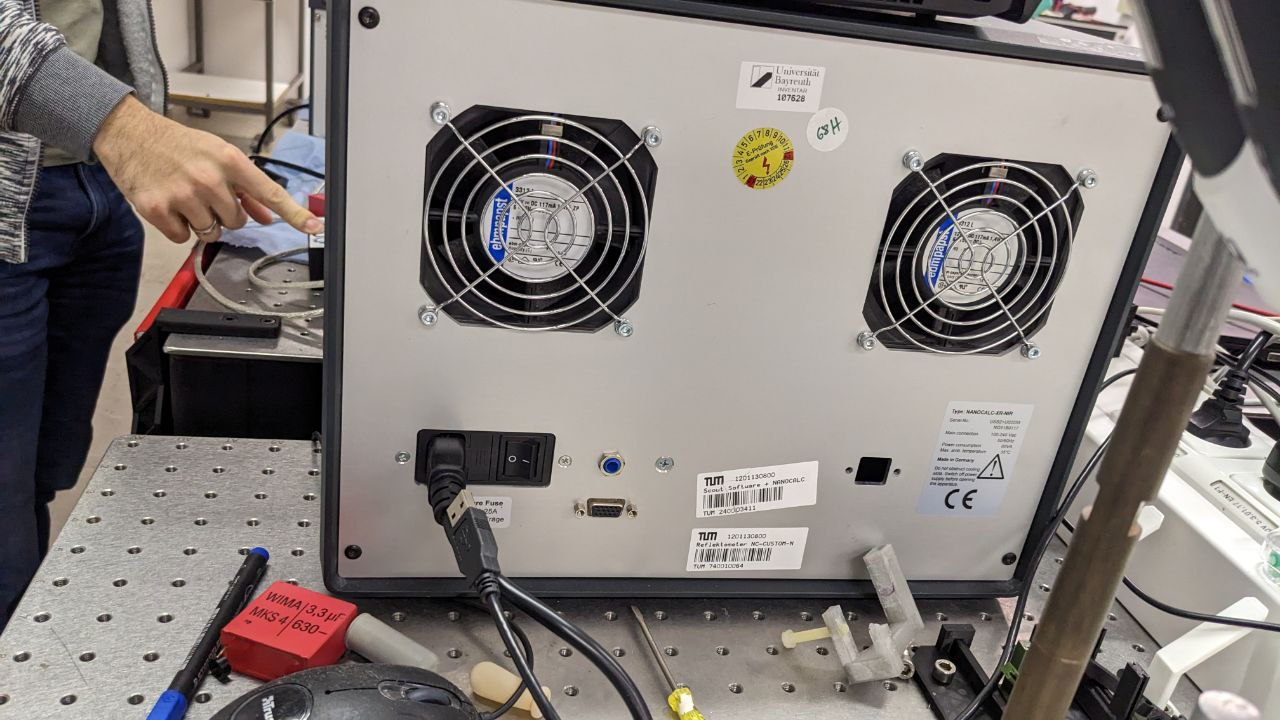
\includegraphics[scale = 0.15]{Lichtquelle-hinten.jpg}
	\end{tabular}
	\captionof{figure}{Halogen-Deuterium-Lampe (links Vorderansicht, rechts Hinteransicht)}
	\label{fig:lampe}
\end{center}
\newpage
Von der Halogen-Deuterium-Lampe gehen Glasfaserkabel zum Aufbau für die Reflexions und Transmissionsmessung [Abb. \ref{fig:mess}].
\begin{center}
	\captionsetup{type=figure}
	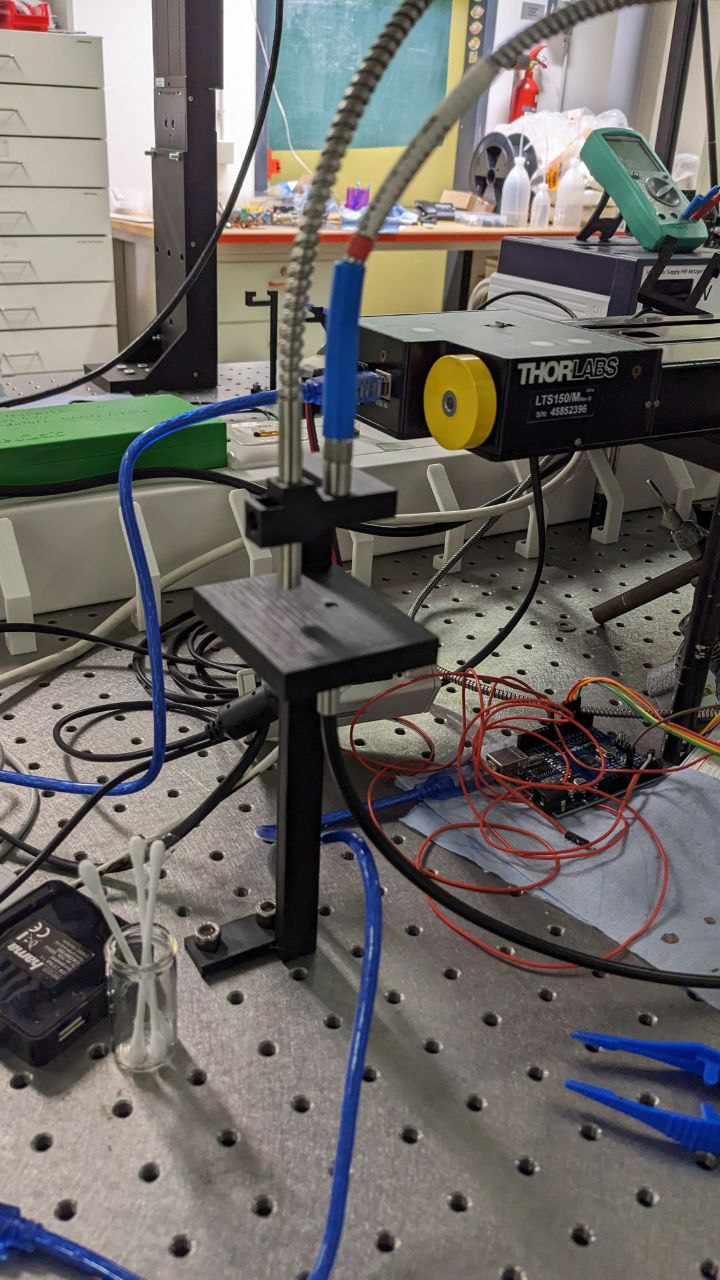
\includegraphics[scale = 0.15]{Messaufbau.jpg}
	\captionof{figure}{Messaufbau (links Reflexion, rechts Transmission)}
	\label{fig:mess}
\end{center}
Das Signal wird wiederum wieder von eine \textit{OceanOptics} Schnittstelle [Abb. \ref{fig:schnitt}] an den PC gesendet und von dem Messprogramm \textit{NanoCalc} ausgewertet.
\begin{center}
	\captionsetup{type=figure}
	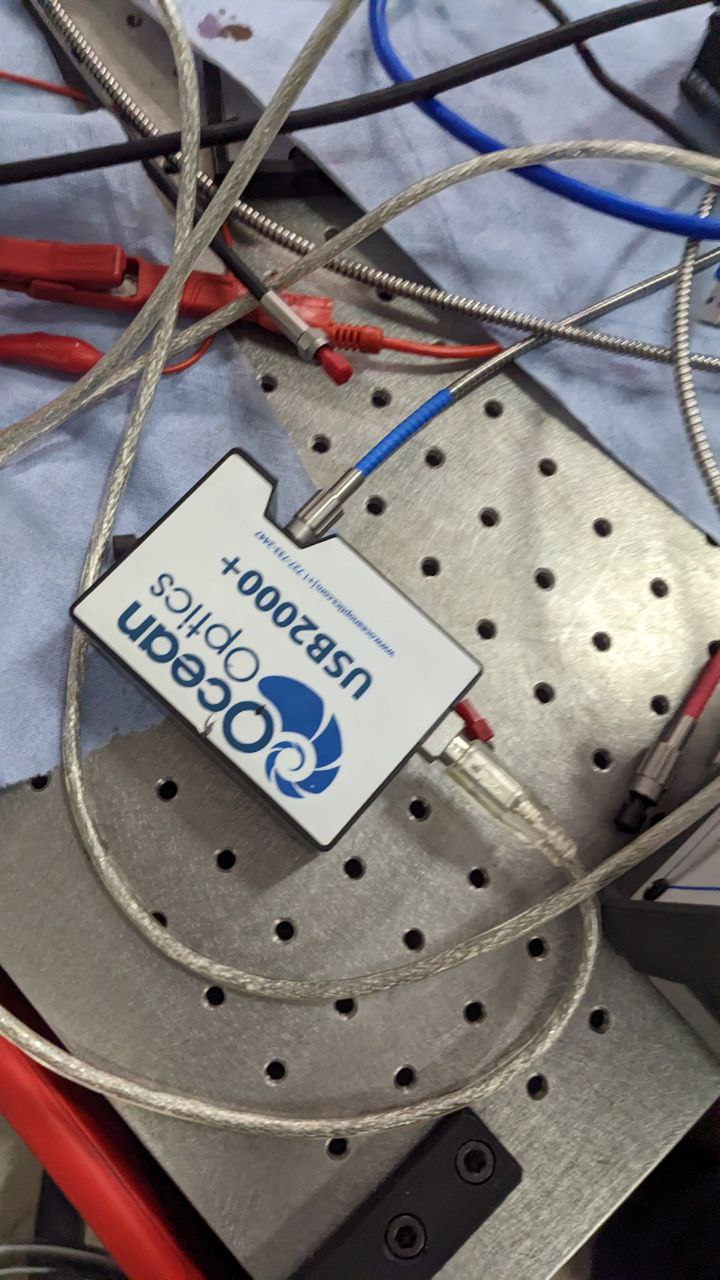
\includegraphics[scale = 0.15]{Schnittstelle.jpg}
	\captionof{figure}{Mikrocontroller zum verarbeiten des Signals}
	\label{fig:schnitt}
\end{center}
\newpage
Für alle Messungen wird die Probe \textit{19} als Referenzprobe genommen. Die Proben mit unterschiedlicher Konzentration werden 6 mal gemessen an 6 verschiedenen auf der Probe.\bigskip

Die Daten werden nach dem Schema:\\
\textit{(Konzentration)mg\_ml\_(Messungsnummer).xy}\\
und später in csv Dateien umgewandelt und umbenannt nach dem Schema:
\begin{itemize}
	\item \textit{Reflexion\_(Konzentration)mg\_ml\_(Messungsnummer).csv}
	\item \textit{Transmission\_(Konzentration)mg\_ml\_(Messungsnummer).csv}
\end{itemize}

Das Programm \textit{NanoCalc} fittet auch sofort für die gemessenen Werte die Dicke $d$ in \si{\nano\metre} mit einem Parameter names Fitness, was eine Güte für den Fit ist. Die jeweiligen werte wurden in:
\begin{itemize}
	\item \textit{Reflexion\_(Konzentration)mg\_ml\_Fit.csv}
	\item \textit{Transmission\_(Konzentration)mg\_ml\_Fit.csv}
\end{itemize}
gespeichert. Dabei ist zu erwähnen, dass das Programm für die Konzentration von \SI{1}{\milli\gram\per\milli\litre} keinen Fit mehr machen konnte. \bigskip

Weiterhin wurden die Integrationszeit, boxcar und die Anzahl der Messung bevor gemittelt (Sample) wird für jede Messart geändert, welche in Tabelle \ref{tab:messPara} gegeben sind.
\begin{center}
	\captionsetup{type=table}
	\begin{tabular}{l | c c c}
		             & Integrationszeit/\si{\milli\sec} & boxcar/pixel & Sample \\
		\hline
		Reflexion    & 25								   & 1				 & 150    \\
		Transmission & 7								   & 1 				 & 600    
	\end{tabular}
	\caption{Veränderte Parameter in \textit{NanoCalc}}
	\label{tab:messPara}
\end{center} 

    % 4.Kapitel Versuchsauswertung
    % 4. Versuchsauswertung

\chapter{Auswertung und Diskussion}
\label{chap:versuchsauswertung}

% Text

% Input der Teilauswertung je nach Produktion der Nebendateien ohne Ordner
% Teilauswertung 1

\section{Einfluss der Messmethode }
\label{sec:mess}

\subsection{Verlauf der Reflexions- und Transmissionsmessung}
\label{sub:verlauf}

Zuerst wird der Einfluss der Konzentrationsvariation auf die Reflexion und Transmission untersucht. 
Dabei wird der Verlauf beider Messungen graphisch dargestellt in Abb. \ref{fig:reflexionVerlauf} den der Reflexionsmessung und in Abb. \ref{fig:transmissionVerlauf} den der Transmissionsmessung. Um die verläufe graphisch darzustellen wurde aus allen 6 Messungen der gleiche Bereich ausgewählt und der Mittelwert über die Amplitude des Signals gebildet.
\begin{center}
	\captionsetup{type=figure}
	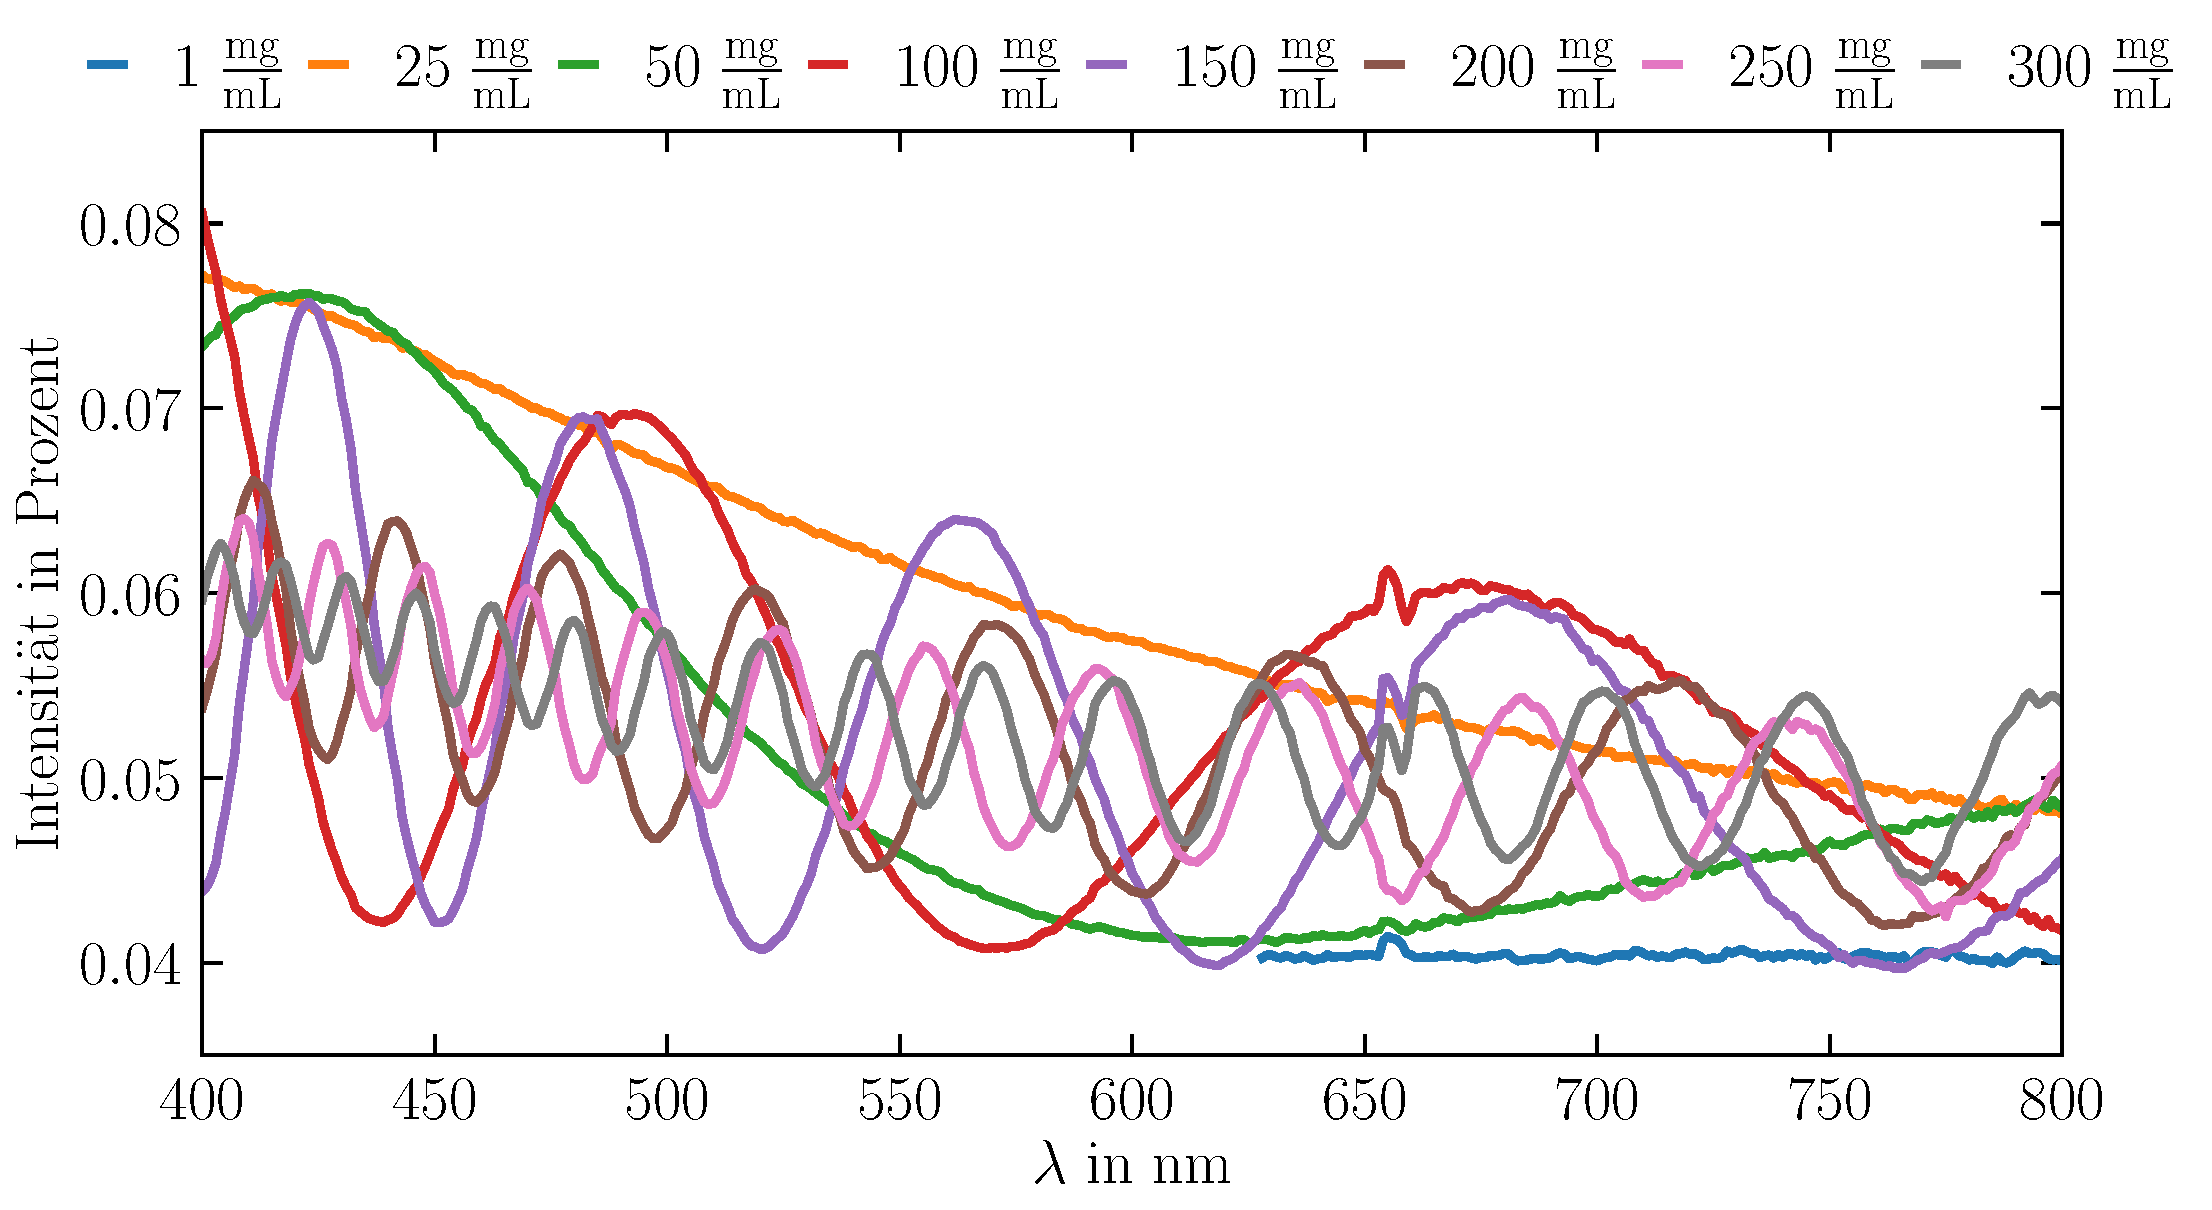
\includegraphics[width=\textwidth]{Auswertung/41/Reflexion.pdf}
	\captionof{figure}{Verlauf der Reflexionsmessung}
	\label{fig:reflexionVerlauf}
\end{center}
Mit Gleichung \ref{eq:wavelength} lässt sich schlussfolgern, dass die Schichtdicke mit zunehmender Konzentration zunimmt. Dies wird verdeutlicht, wenn man die Differenz zweier benachbarten Maximas im Spektrum. Dafür stellen wir Gleichung \ref{eq:wavelength} der reflektierten Welle (mit transmittierter Welle analog) für die Beugungsordnung $m$ um:
\begin{gather}
	\left(m_1 + \frac{1}{2}\right) - \left(m_2 + \frac{1}{2}\right) = 2nd \left(\frac{1}{\lambda_1} - \frac{1}{\lambda_2}\right)~.
\end{gather}
Da $m_1$ und $m_2$ benachbarte Maxima sind ergibt die Differenz einfach nur 1, zusammen mit dem Wellenlängenunterschied $\Delta \lambda = \lambda_2 - \lambda_1$ ergibt sich:
\begin{gather}
	\boxed{\frac{\lambda_1\lambda_2}{\Delta\lambda} = 2nd \Rightarrow d \xrightarrow{\Delta \lambda \rightarrow 0} \infty}~.
\end{gather} 
Dieser Zusammenhang zeigt, je kleiner der Wellenlängenunterschied $\Delta \lambda$ wird, desto größer ist die Schichtdicke $d$. Deswegen lässt sich aus Abb. \ref{fig:reflexionVerlauf} und Abb. \ref{fig:transmissionVerlauf} erkennen, dass mit zunehmender Konzentration die Schichtdicke $d$ zunimmt, da der Wellenlängenunterschied $\Delta \lambda$ kleiner wird.
\begin{center}
	\captionsetup{type=figure}
	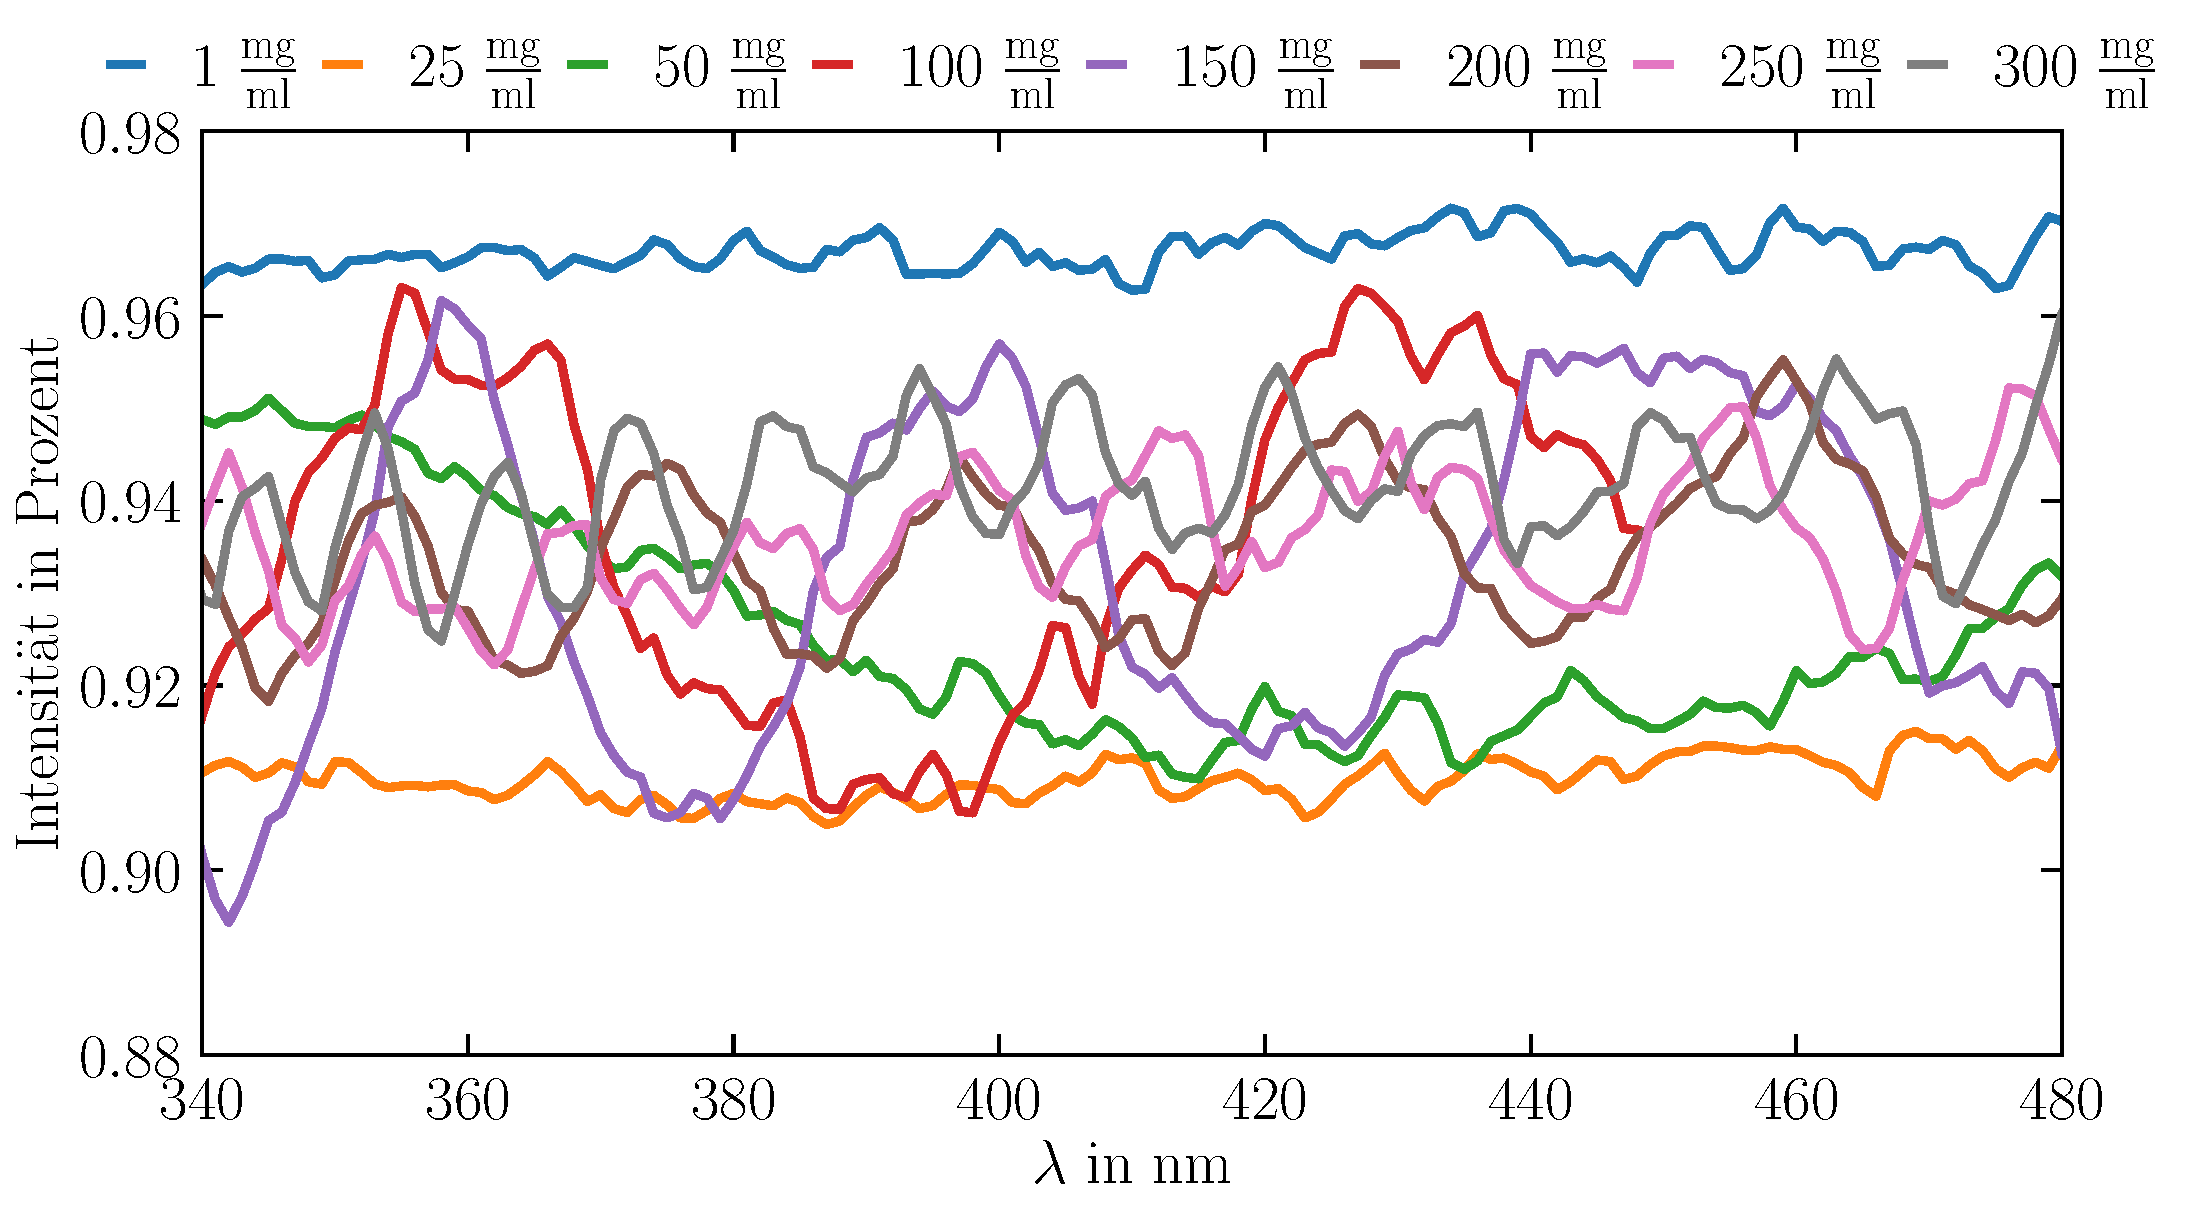
\includegraphics[width=\textwidth]{Auswertung/41/Transmission.pdf}
	\captionof{figure}{Verlauf der Transmissionsmessung}
	\label{fig:transmissionVerlauf}
\end{center}

\subsection{Hetrogenität $h$ der Probe}
\label{sub:fitguete}

Als nächstes betrachten wir die Heterogenität $h$ der Probe, um daraus die Homogenität dieser zu bestimmen. Dafür wir die Heterogenität $h$ mit folgender Formel berechnet:
\begin{gather}
	\boxed{h = \frac{\langle d \rangle}{std(d)}}~, 
\end{gather}
wobei $\langle d \rangle$ der Mittelwert und $std(d)$ die Standardabweichung der Schichtdicke $d$ für jede einzelne Probe ist. Als Werte für die Statistik werden die aufgenommenen Daten des NanoCalc Programms verwendet. Weiterhin wird auch die Fitgüte $\chi$ aus den Programm auch gemittelt ($\langle\chi\rangle)$. Die Ergebnisse werden in Tab. \ref{tab:homogen} dargestellt und wurden mit der \textit{mean()} und \textit{std()} Funktion des \textit{python}-Modules \textit{pandas} berechnet. 
\begin{center}
	\captionsetup{type=table}
	\begin{tabular}{c}	
		\begin{tabular}{r | r r r | r}
			$c$/\si{\milli\gram\per\milli\litre} & $\langle d \rangle$/\si{\nano\metre} & $std(d)$/\si{\nano\metre} & $h$ & $\langle \chi \rangle$ \\[0,1cm]
			\hline
			300 & 3656.3 & 33.1 & 110.5 & 0.016024 \\
			250 & 2708.4 & 33.1 &  81.8 & 0.016509 \\
			200 & 1702.4 & 20.0 &  85.1 & 0.011317 \\
			150 &  975.0 &  3.7 & 263.5 & 0.007943 \\
			100 &  539.2 &  3.6 & 149.8 & 0.007949 \\
			 50 &   60.6 &  1.0 &  60.6 & 0.005747 \\
			 25 &   60.6 &  1.0 &  60.6 & 0.005688 \\
		\end{tabular} \\[2cm]
		\begin{tabular}{r | r r r | r}
			$c$/\si{\milli\gram\per\milli\litre} & $\langle d \rangle$/\si{\nano\metre} & $std(d)$/\si{\nano\metre} & $h$ & $\langle \chi \rangle$ \\[0,1cm]
			\hline
			300 & 3756.9 & 23.2 & 161.9 & 0.101230 \\
			250 & 2835.6 & 37.5 &  75.6 & 0.093220 \\
			200 & 1833.5 & 24.3 &  75.5 & 0.101994 \\
			150 &  981.4 &  5.3 & 185.2 & 0.203744 \\
			100 &  564.1 & 41.1 &  13.7 & 0.299021 \\
			 50 &  200.1 &  7.3 &  27.4 & 0.214980 \\
			 25 &   64.1 &  1.5 &  42.7 & 0.435492 \\
		\end{tabular} \\
	\end{tabular}
	\captionof{table}{Werte für Homogenität bei Reflexion (oben) und Transmission (unten)}
	\label{tab:homogen}
\end{center}
In Tab. \ref{tab:homogen} lässt durch die Heterogenität $h$ sehen, dass die Probe selber nur wenig homogen verteilt ist. Dies bedeutet, dass sich einige dichtere Stellen von Material auf der Probe gebildet haben. Jedoch je höher die Konzentration war, desto homogener wurde der Dünnfilm auf der Probe. Anzumerken ist noch, dass die Hetrogenität $h$ der Transmission am aussagekräftigsten ist, da für das Messsignal das Licht der Halogen-Deuterium-Lampe durch die ganze Probe laufen muss. \bigskip

\subsection{Schichtdicke $d$ der Proben im Vergleich zur Fitgüte $\chi$}
\label{sub:fitguete}

Im nächsten Schritt wird der Mittelwert der Fitgüte $\langle \chi \rangle$ mit den Mittelwert und der Schichtdicke $\langle d \rangle$ und der Standardabweichung der Schichtdicke  $std(d)$ verglichen. In Abb. \ref{fig:fitgueteReflexion} und Abb. \ref{fig:fitueteTransmission} wird dieser Zusammenhang graphisch mit den Werten aus Tab. \ref{tab:homogen} dargestellt. Dabei lässt sich erkennen, dass bei der Reflexion die Verläufe linearer Proportionalität und bei der Transmission indirekter Proportionalität sind. Ein Fit mit der \textit{curve\_fit()} Funktion aus dem \textit{python}-Modules \textit{scipy.optimize} ergibt dann folgende Werte in Tab. \ref{tab:fitgueteFit}
\begin{center}
	\captionsetup{type=table}
	\begin{tabular}{l | c c | c c}
		  & \multicolumn{2}{c |}{Reflexion} &\multicolumn{2}{c}{Tranmission} \\
		  & $\langle \chi \rangle = a\,\langle d \rangle  + b$ & $\langle \chi \rangle = a\,std(d)  + b$ & $\langle \chi \rangle = a/\langle d \rangle^2 + b$ & $\langle \chi \rangle = a/std(d)^2 + b$\\
		  \hline
		  $a$/\si{\per\nano\metre} & 0.000003 & 0.000304 &  1.34 &  0.77 \\
		  $b$                      & 0.005714 & 0.006008 & -0.39 & -0.36 \\
	\end{tabular}
	\captionof{table}{Ermittelte Fitparameter für Reflexion- und Transmissionsmessung}
	\label{tab:fitgueteFit}
\end{center}
Es zeigt sich, dass die Fitgüte $\chi$ je nach Art der Messung verschieden skaliert abhängig von der Konzentration auf der Probe und damit der Schichtdicke $d$. \\
Dabei weißen Reflexion und Transmission gegenläufige Ergebnisse auf, dass sich sich in den Verläufen in Abb. \ref{fig:fitgueteReflexion} und Abb. \ref{fig:fitueteTransmission} erkennen lässt. Für die Reflexion ist hierbei die Fitgüte $\chi$ maximal, wenn die Schichtdicke $d$ groß ist, während für die Transmission die Fitgüte $\chi$ minimal ist für große Schichtdicken $d$. 
\begin{center}
	\captionsetup{type=figure}
	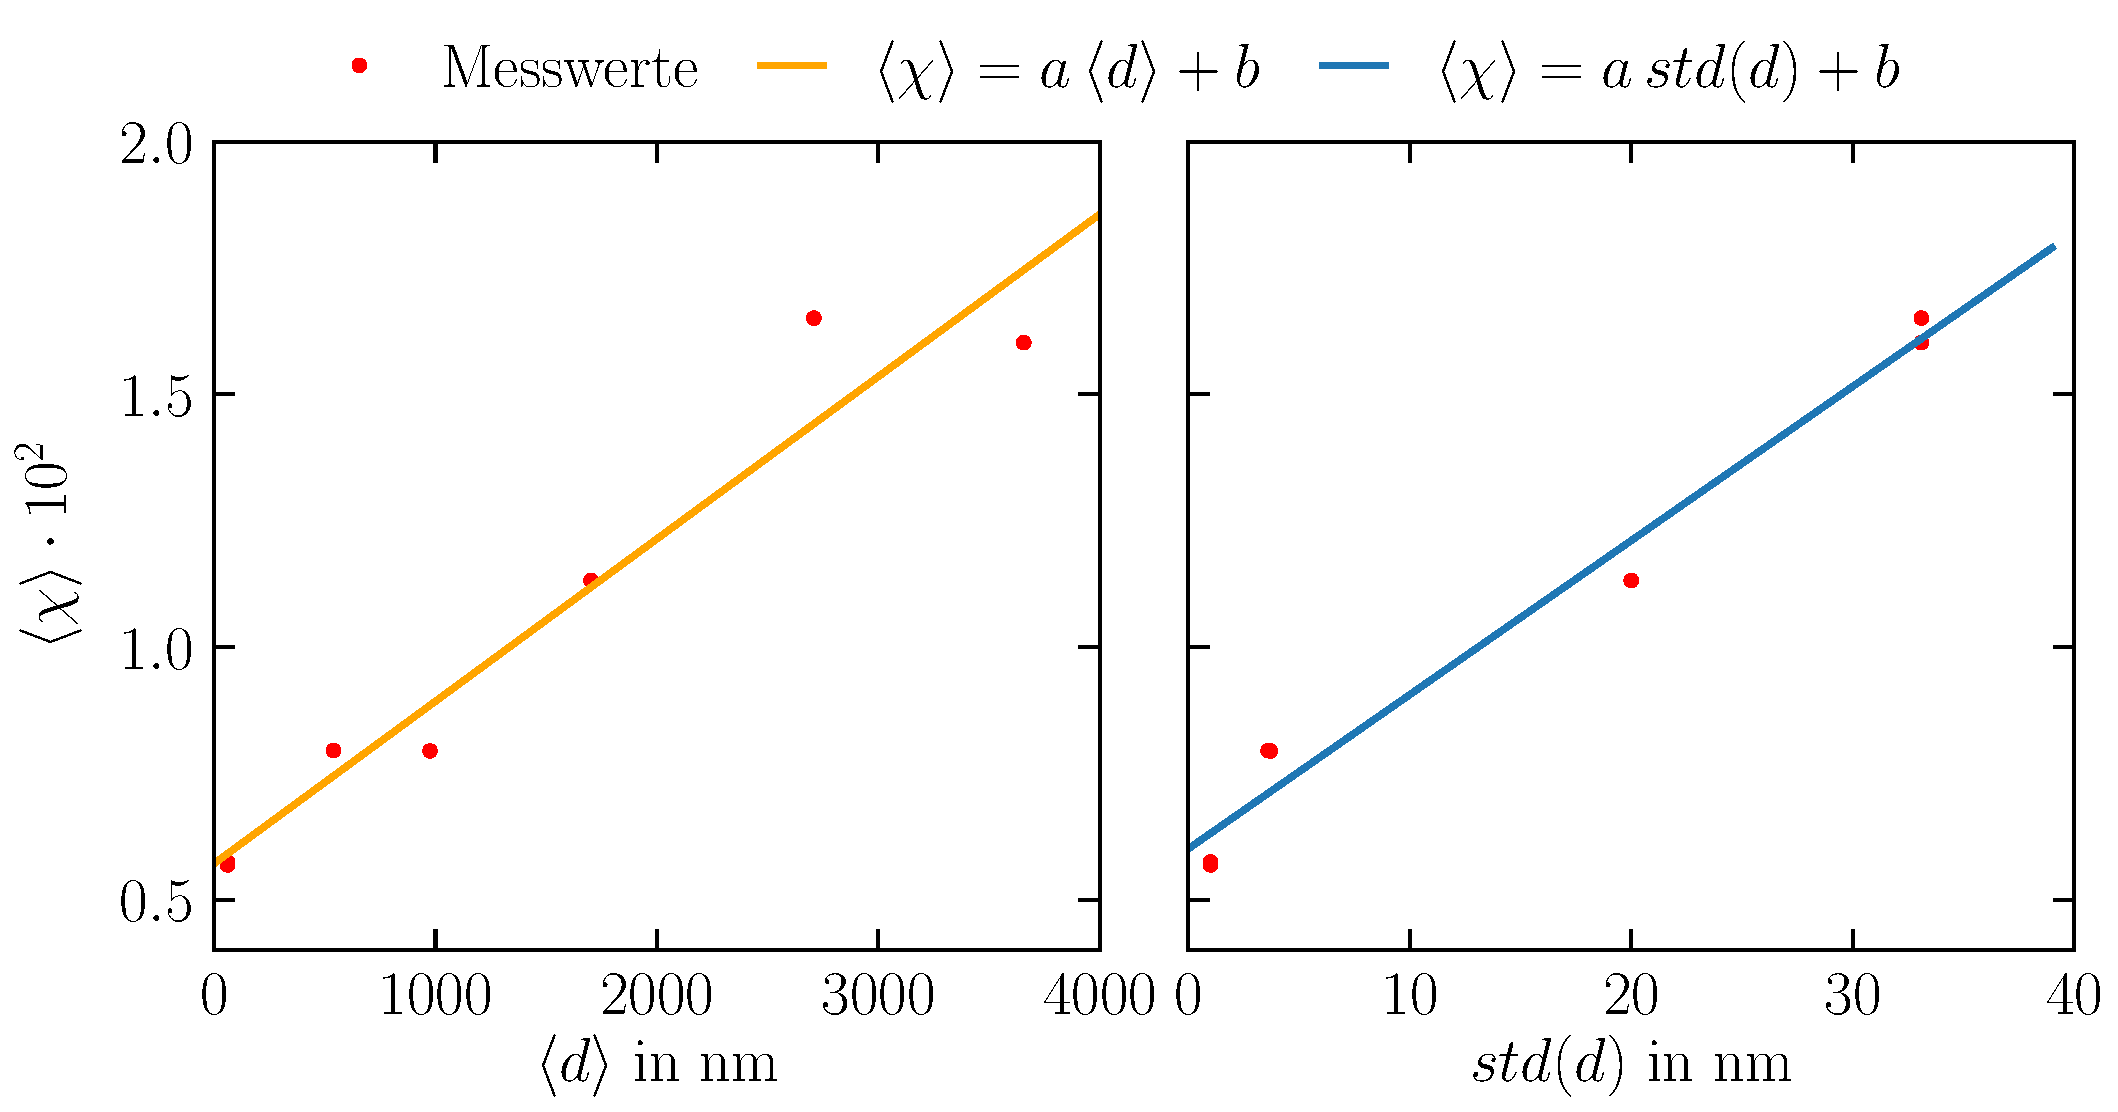
\includegraphics[width=0.92\textwidth]{Auswertung/41/Reflexion-Fitguete.pdf}
	\captionof{figure}{Mittelwert und Standardabweichung der Schichtdicke $d$ aufgetragen gegen den Mittelwert der Fitgüte $\langle \chi \rangle$ bei Reflexion}
	\label{fig:fitgueteReflexion}
\end{center}
\begin{center}
	\captionsetup{type=figure}
	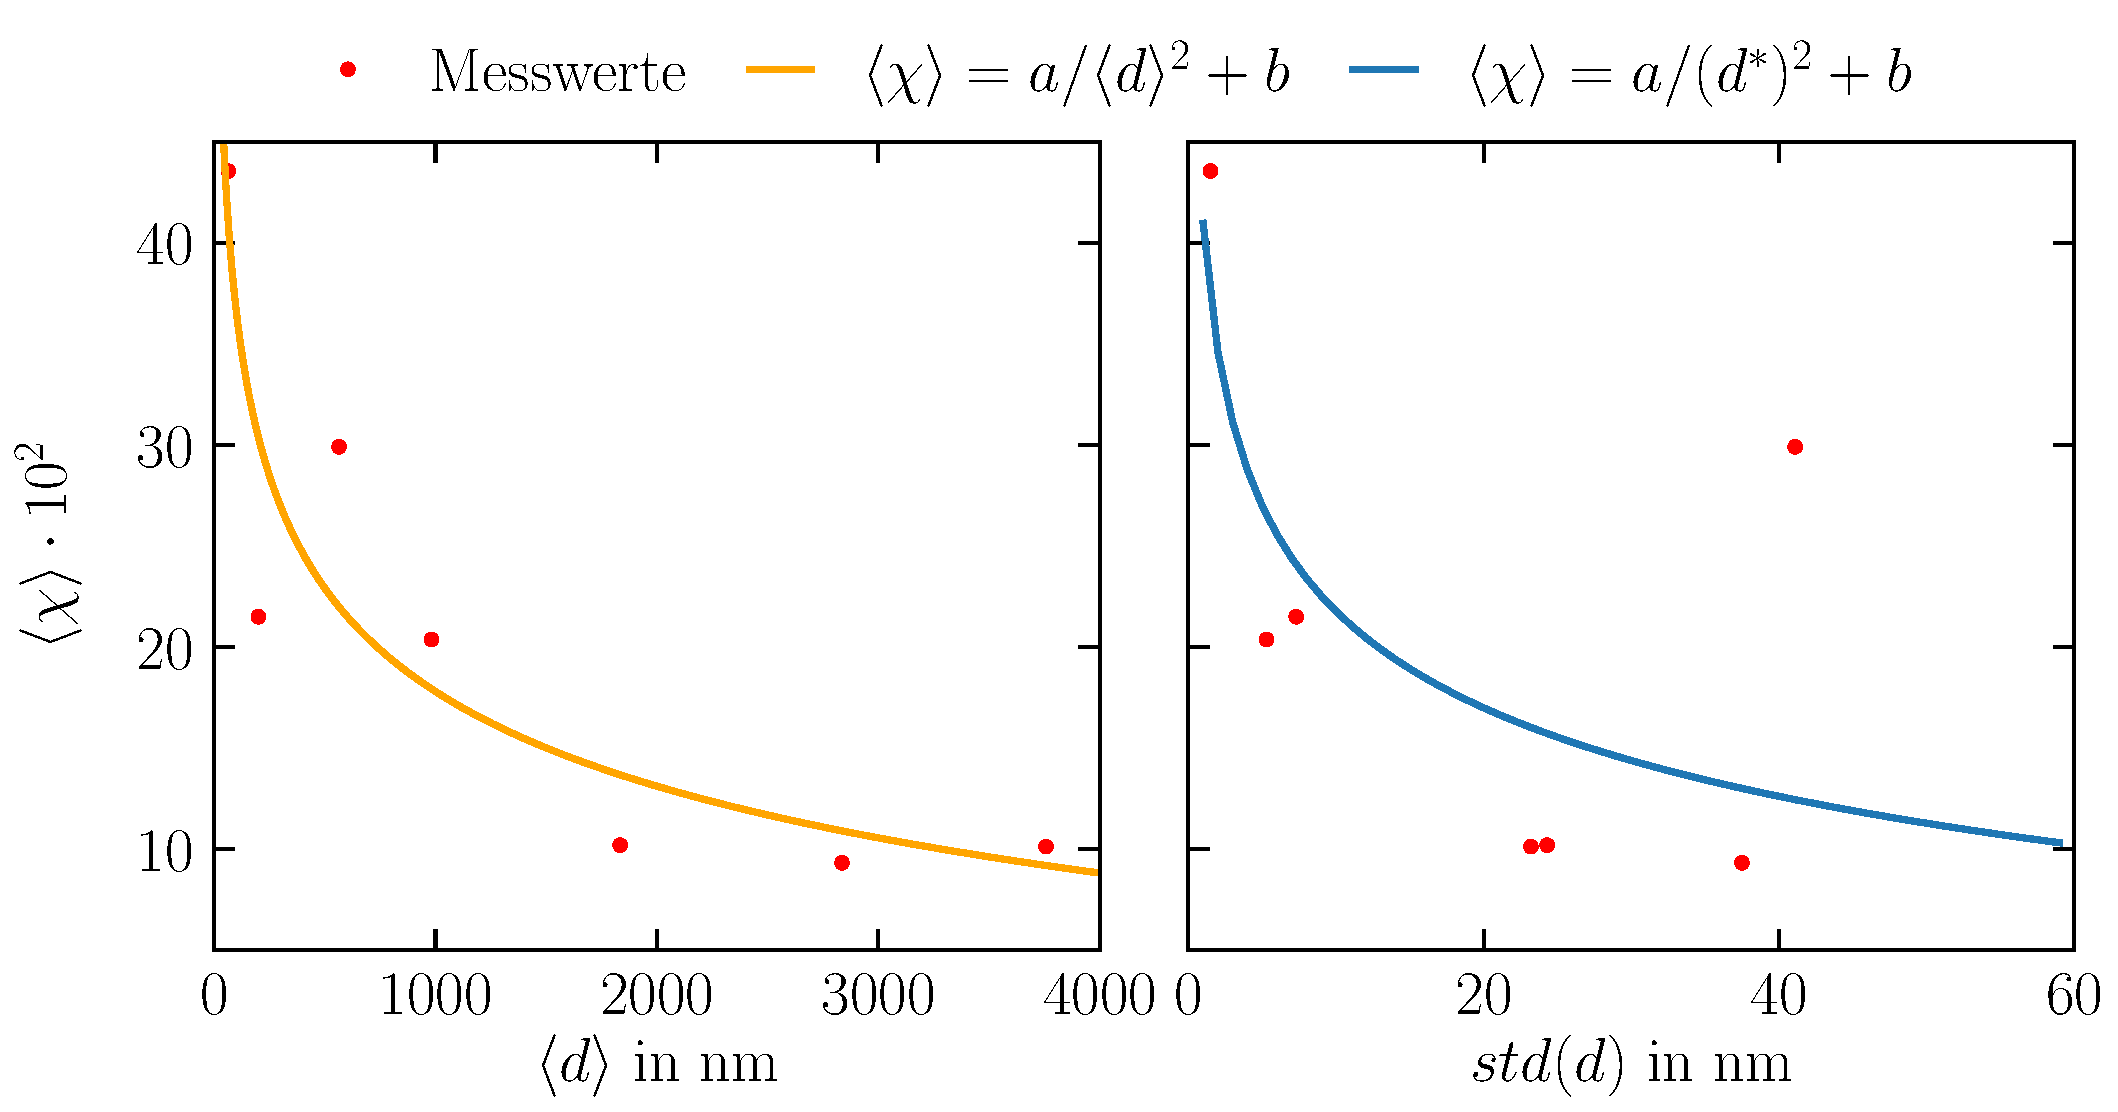
\includegraphics[width=0.92\textwidth]{Auswertung/41/Transmission-Fitguete.pdf}
	\captionof{figure}{Mittelwert und Standardabweichung der Schichtdicke $d$ aufgetragen gegen den Mittelwert der Fitgüte $\langle \chi \rangle$ bei Transmission}
	\label{fig:fitueteTransmission}
\end{center}


\subsection{Vergleich der Messmethoden}
\label{sub:vergleich}

Tab. \ref{tab:homogen} zeigt, dass bei Reflexion und Transmission ähnliche Werte für die Schichtdicke $d$ gemessen werden. Jedoch ist die Messung der Reflexion mit einem besseren Signal möglich als bei der Transmission [Fig. \ref{fig:reflexionVerlauf}, \ref{fig:transmissionVerlauf}]. Auch liefert die Reflexionsmessung einen linearen Zusammenhang [Fig. \ref{fig:fitgueteReflexion}] zwischen Fitgüte $\chi$ und der Schichtdicke $d$, was eine klare Prognose für die Fits der NanoCalc Software verspricht. Dennoch kann die Transmissionsmessung, dafür genutzt werden die Hetreogenität und damit die Homogenität der Probe zu bestimmen und ist der der Messung mit Reflexion vorzuziehen.
% Teilauswertung 2
\newpage
\section{Dunkelfeldspektroskopie einer Nanorodprobe}
\label{sec:nanorods}

\begin{center}
    \captionsetup{type = figure}
    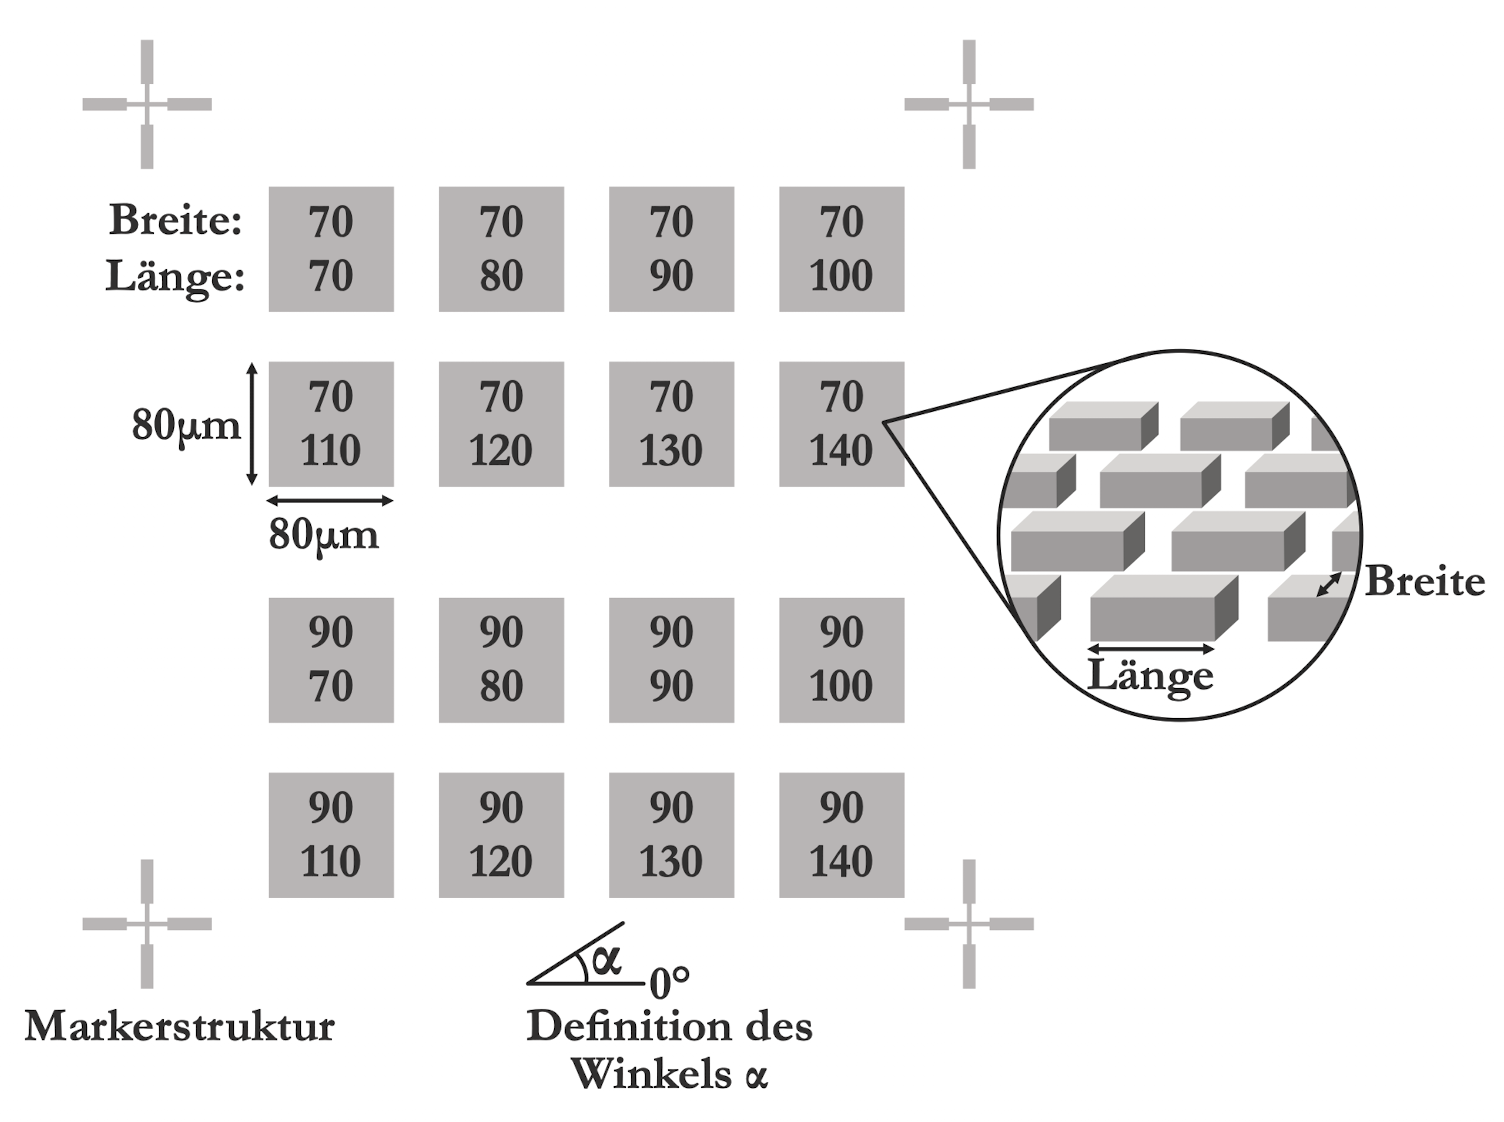
\includegraphics[width = \textwidth]{Bilder/Nanorods.png}
    \captionof{figure}{
        Übersichtsplan der verwendeten Probe. Die gesamte Probenstruktur befindet sich mehrmals auf einem Glassubstrat. Die Struktur selbst besteht aus Markern und 16 Feldern, die jeweils tausende Nanorod gleicher Dimensionen enthalten. Die Breite und Länge der Partikel in Nanometern sind auf den Feldern eingetragen. Das Inset zeigt die Vergrößerung eines einzelnen Probenfelds, wodurch die Orientierung der langen Achse der Rods und die Definition von Breite und Länge erkennbar ist. Der Winkel $\alpha$ ist unter dem Übersichtsplan definiert. Eine Polarisation von $\alpha = 0^\circ$ führt damit zu einer Anregung entlang der langen Achse der Rods. \cite{Anleitung}
    }
    \label{fig:nanorods}
\end{center}

In diesem Versuchsteil wurden mehrere Struktuten mit unterschiedlicher Nanorods (bestehend aus Silber) mit einer Breite von 70\,nm und 90\,nm und variabler Länge $L$ untersucht. Abbildung \ref{fig:nanorods} zeigt hierbei den Übersichtsplan der Probe, mit dem Parameter der Rods in den einzelnenFelder. Jedes Feld hat eine Größe von 80$\times$80\,$\mu$m und beinhaltet tausende identische Nanorods, womit das Streuspektrim aller Rods auf einem Feld gemessen werden kann. Der Winkel $\alpha$ gibt folgenden die Richtung der Polarisation an, wobei $\alpha = 0^\circ$ die Länge der Rods anregt und $\alpha = 90^\circ$ die Breite der Rods. \cite{Anleitung}

Es wurden einerseites die Spektren der Nanorods mit Intensität $I_\mathrm{N}$ als auch ein Dunkelspektrum $I_\mathrm{D}$ und ein Referenzspektrum $I_\mathrm{R}$ am Anfang und am Ende der Messung aufgenommen. Da in beiden Messungen das Dunkelspektrum mitgemessen wurde, wird dieses in der weiteren Rechnung nicht mehr beachtet (siehe auch Kapitel \ref{sub:korrigiertesSignal}). Um ein korrigieres Dunkelfeldspektrum $I_\mathrm{C}$ zu erhalten wird folgende Formel angewendet
\begin{gather}
    I_\mathrm{C} = \frac{I_\mathrm{N}}{\langle I_\mathrm{R} \rangle} ~,
\end{gather}
wobei $\langle I_\mathrm{R} \rangle$ der Mittelwert zwischen dem Referenzspektrum am Anfang und am Ende der Messung ist. Das korrigierte Dunkelfeldspektrum $I_\mathrm{C}$ (Einheit a.u. = arb. units) wurde in Abb. \ref{fig:spektrum} in Abhängigkeit der Wellenlänge $\lambda$ (Einheit nm) dargestellt. Dabei lässt sich für unpolarisiertes und polarisiertes Licht ($\alpha = 0^\circ$) erkennen, dass für zunehmende Rodlänge die Intensität $I_\mathrm{C}$ abnimmt. Für $\alpha = 90^\circ$ Polarisation ist dieser Effekt nur bei einer Rodbreite von 70\,nm zu erkennen, wobei hier zwei Maxima beobachtet werden können, welche selbst konstant sind für gewisse Rodlängen. Für eine Rodbreite von 90\,nm ist die Intensität unabhängig von der Rodlänge. Da erwartet wurde, dass sich die Intensität für eine Polarisation von $\alpha = 90^\circ$ nicht ändern sollte, lässt sich vermuten, dass bei der Messung von der Rodbreite 70\,nm ein Messfehler enstanden ist. 
\bigskip
Im nächsten Schritt wird durch einen Gauss-Fit die Maxima der Dunkelfeldspektren bestimmt. Die berechenten Werte können in Tabelle \ref{tab:nanorods} gefunden werden.
\newpage
\begin{sidewaysfigure}
    \centering
    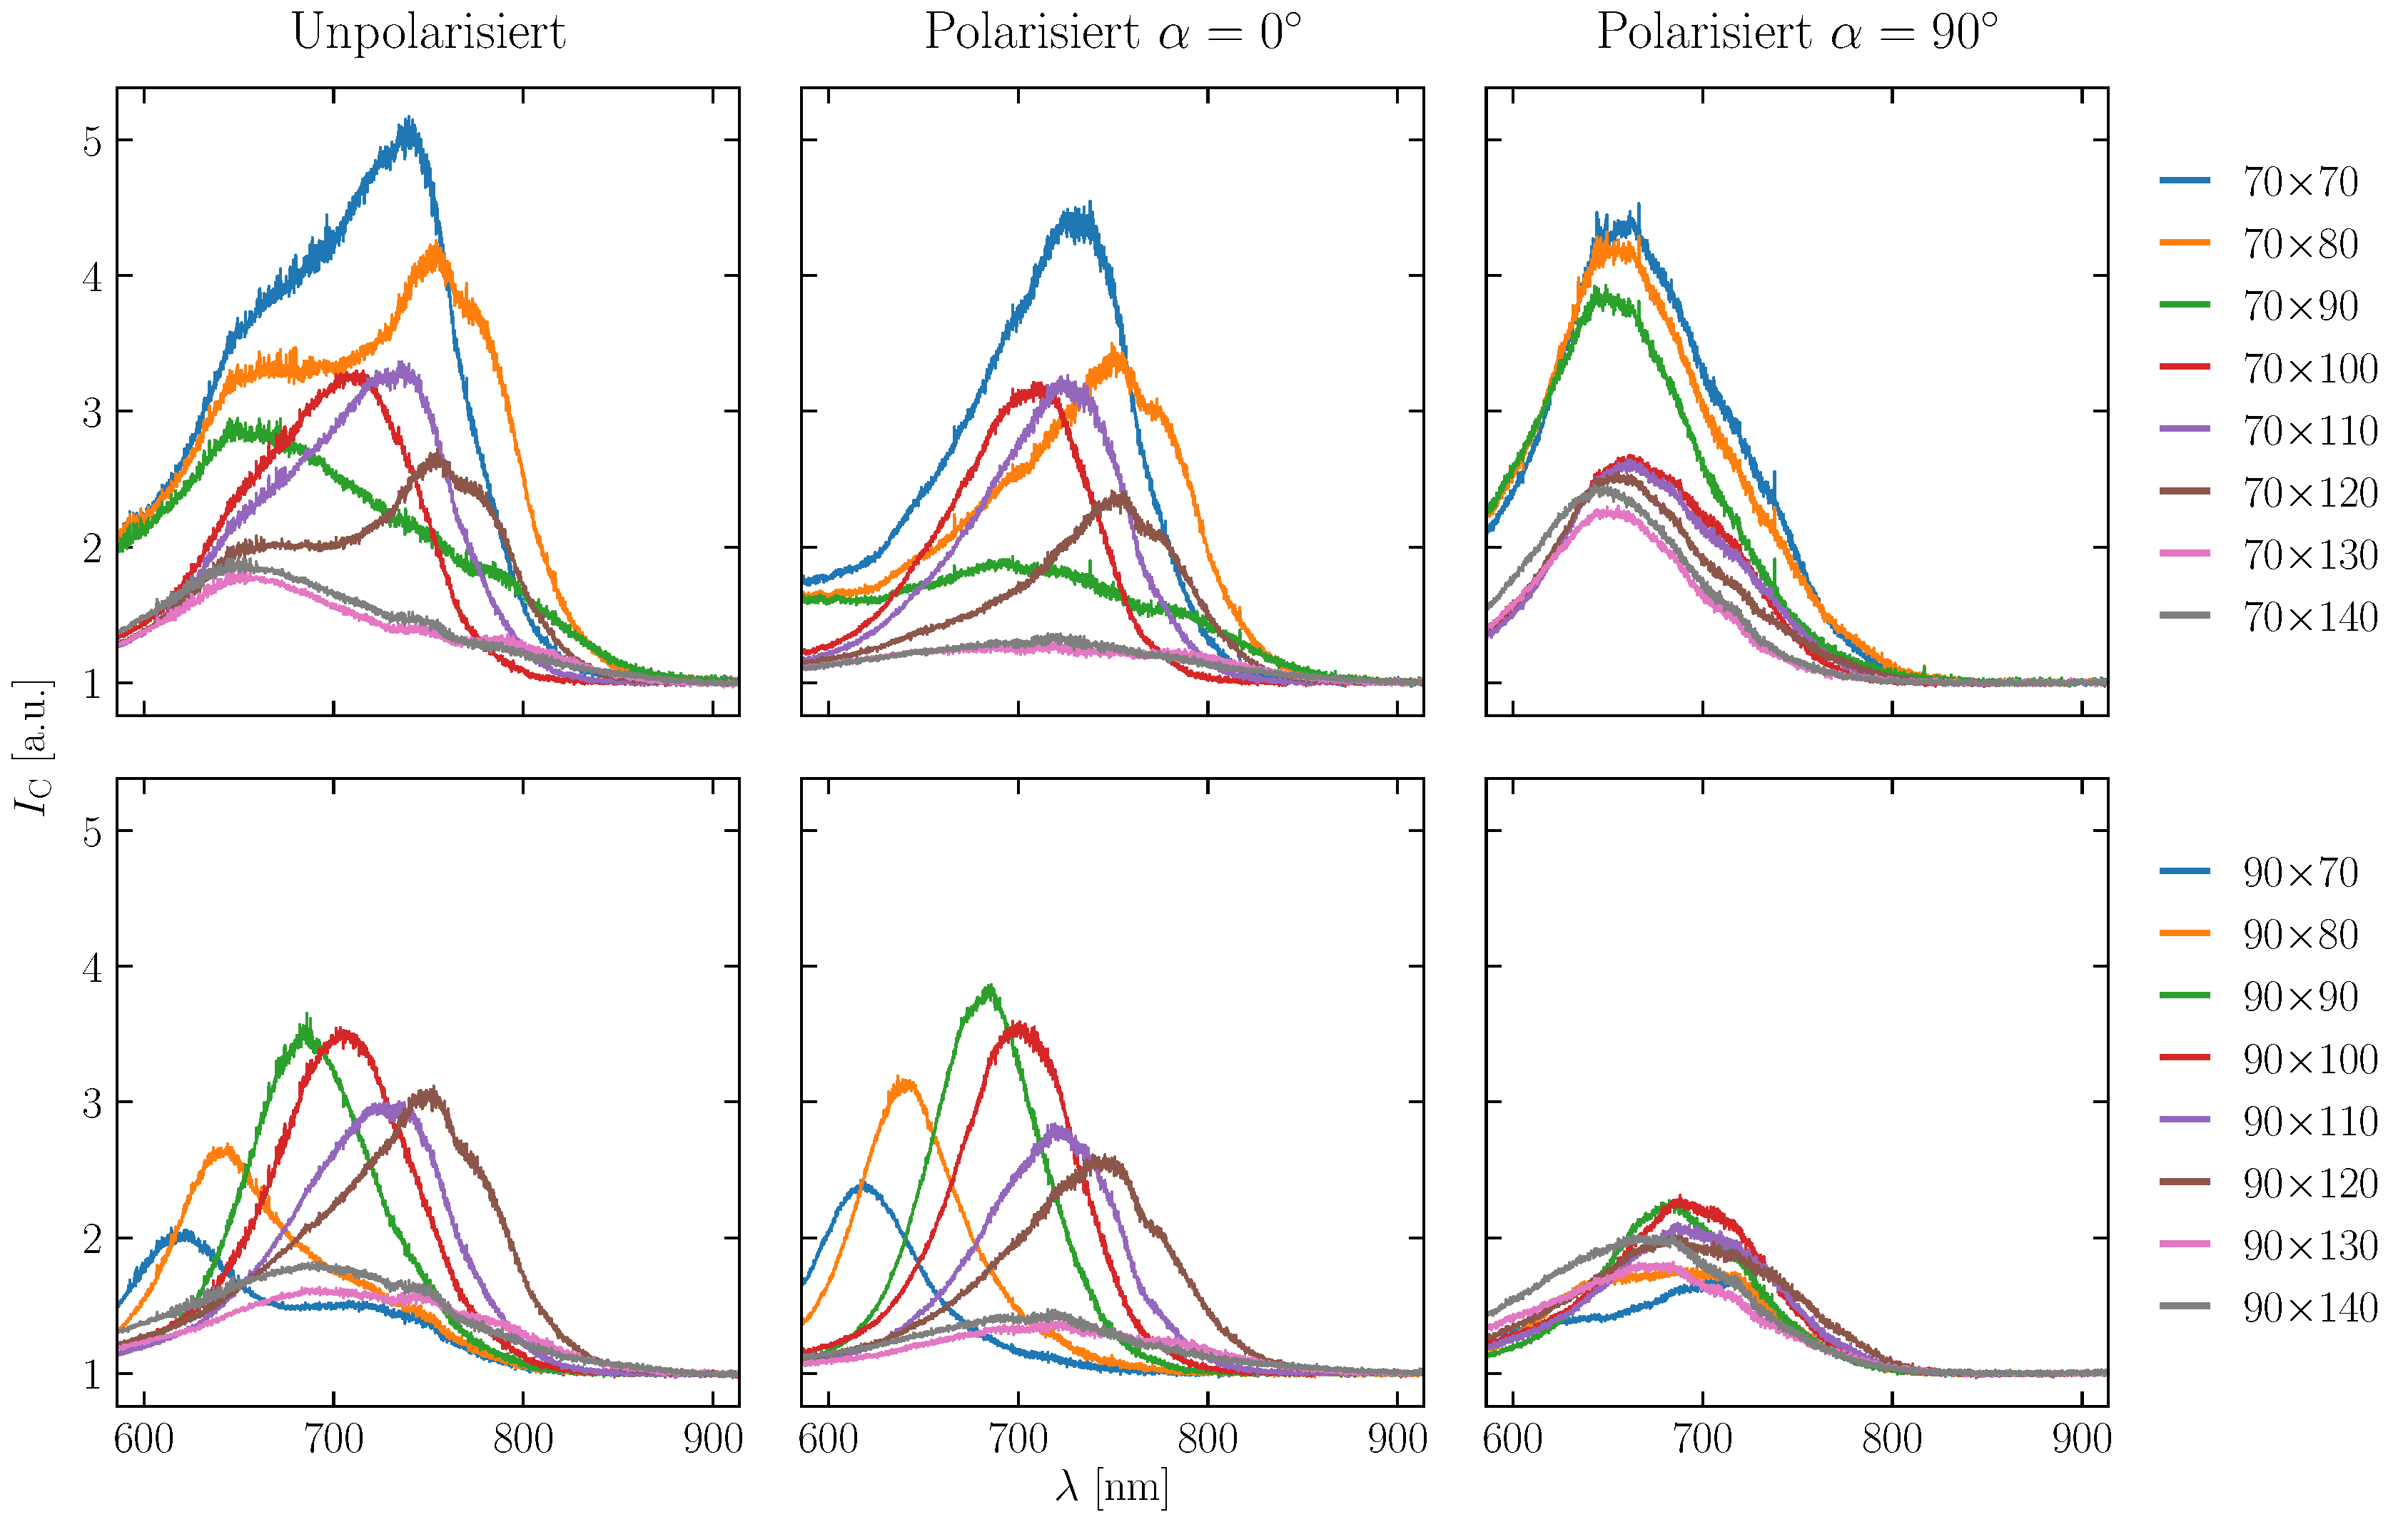
\includegraphics[width = \textheight]{Bilder/Auswertung/3.2/Spektren_Gruppe2.pdf}
    \caption{Korrigiertes Spektrum der Nanorodproben mit unpolarisierten und polarisierten ($\alpha = 0^\circ~;~90^\circ$) Lichtquelle. Die Rodlänge und die Rodbreite in Nanometer wurde mit Nomenklatur Rodbreite$\times$Rodlänge dargestellt}
    \label{fig:spektrum}
\end{sidewaysfigure}

\begin{center}
    \captionsetup{type = table}
    \begin{tabular}{r | c c c}
        $L$/nm & $\tilde{\lambda}^\mathrm{unpol}_{70}$/nm & $\tilde{\lambda}^\mathrm{\alpha = 0^\circ}_{70}$/nm & $\tilde{\lambda}^\mathrm{\alpha = 90^\circ}_{70}$/nm \\\hline
        70  & 704.97 $\pm$ 0.30 & 714.14 $\pm$ 0.25 & 664.06 $\pm$ 0.09 \\
        80  & 711.90 $\pm$ 0.45 & 731.00 $\pm$ 0.35 & 659.14 $\pm$ 0.10 \\
        90  & 670.03 $\pm$ 0.24 & 686.91 $\pm$ 0.28 & 651.89 $\pm$ 0.07 \\
        100 & 696.28 $\pm$ 0.15 & 700.19 $\pm$ 0.12 & 668.09 $\pm$ 0.06 \\
        110 & 711.12 $\pm$ 0.22 & 716.24 $\pm$ 0.15 & 668.05 $\pm$ 0.09 \\
        120 & 722.66 $\pm$ 0.47 & 741.14 $\pm$ 0.26 & 661.00 $\pm$ 0.11 \\
        130 & 669.37 $\pm$ 0.46 & 704.26 $\pm$ 0.34 & 653.20 $\pm$ 0.06 \\
        140 & 664.93 $\pm$ 0.26 & 704.78 $\pm$ 0.17 & 649.43 $\pm$ 0.05 \\
    \end{tabular}\\[0.5cm]
    \begin{tabular}{r | c c c}
        $L$/nm & $\tilde{\lambda}^\mathrm{unpol}_{90}$/nm & $\tilde{\lambda}^\mathrm{\alpha = 0^\circ}_{90}$/nm & $\tilde{\lambda}^\mathrm{\alpha = 90^\circ}_{90}$/nm \\\hline
        70  & 610.84 $\pm$ 1.64 & 619.92 $\pm$ 0.12 & 686.79 $\pm$ 0.29 \\
        80  & 653.88 $\pm$ 0.31 & 642.89 $\pm$ 0.09 & 678.25 $\pm$ 0.14 \\
        90  & 688.00 $\pm$ 0.06 & 683.02 $\pm$ 0.04 & 684.50 $\pm$ 0.06 \\
        100 & 703.85 $\pm$ 0.08 & 699.08 $\pm$ 0.07 & 690.43 $\pm$ 0.10 \\
        110 & 718.89 $\pm$ 0.13 & 716.34 $\pm$ 0.10 & 691.28 $\pm$ 0.09 \\
        120 & 735.59 $\pm$ 0.24 & 734.54 $\pm$ 0.15 & 687.75 $\pm$ 0.10 \\
        130 & 705.59 $\pm$ 0.14 & 714.76 $\pm$ 0.15 & 668.04 $\pm$ 0.09 \\
        140 & 689.79 $\pm$ 0.10 & 699.93 $\pm$ 0.15 & 664.27 $\pm$ 0.08 \\
    \end{tabular}
    \captionof{table}{
        Test
    }
    \label{tab:nanorods}
\end{center}
% Teilauswertung 2

\newpage
\section{Konzentrationsabhängigkeit von Schichtdicken}
\label{sec:konzDicke}
Zuerste werden die ermittelten Schichtdicken gegen die Polymerkonzentration aufgetragen:

\begin{center}
	\captionsetup{type=figure}
	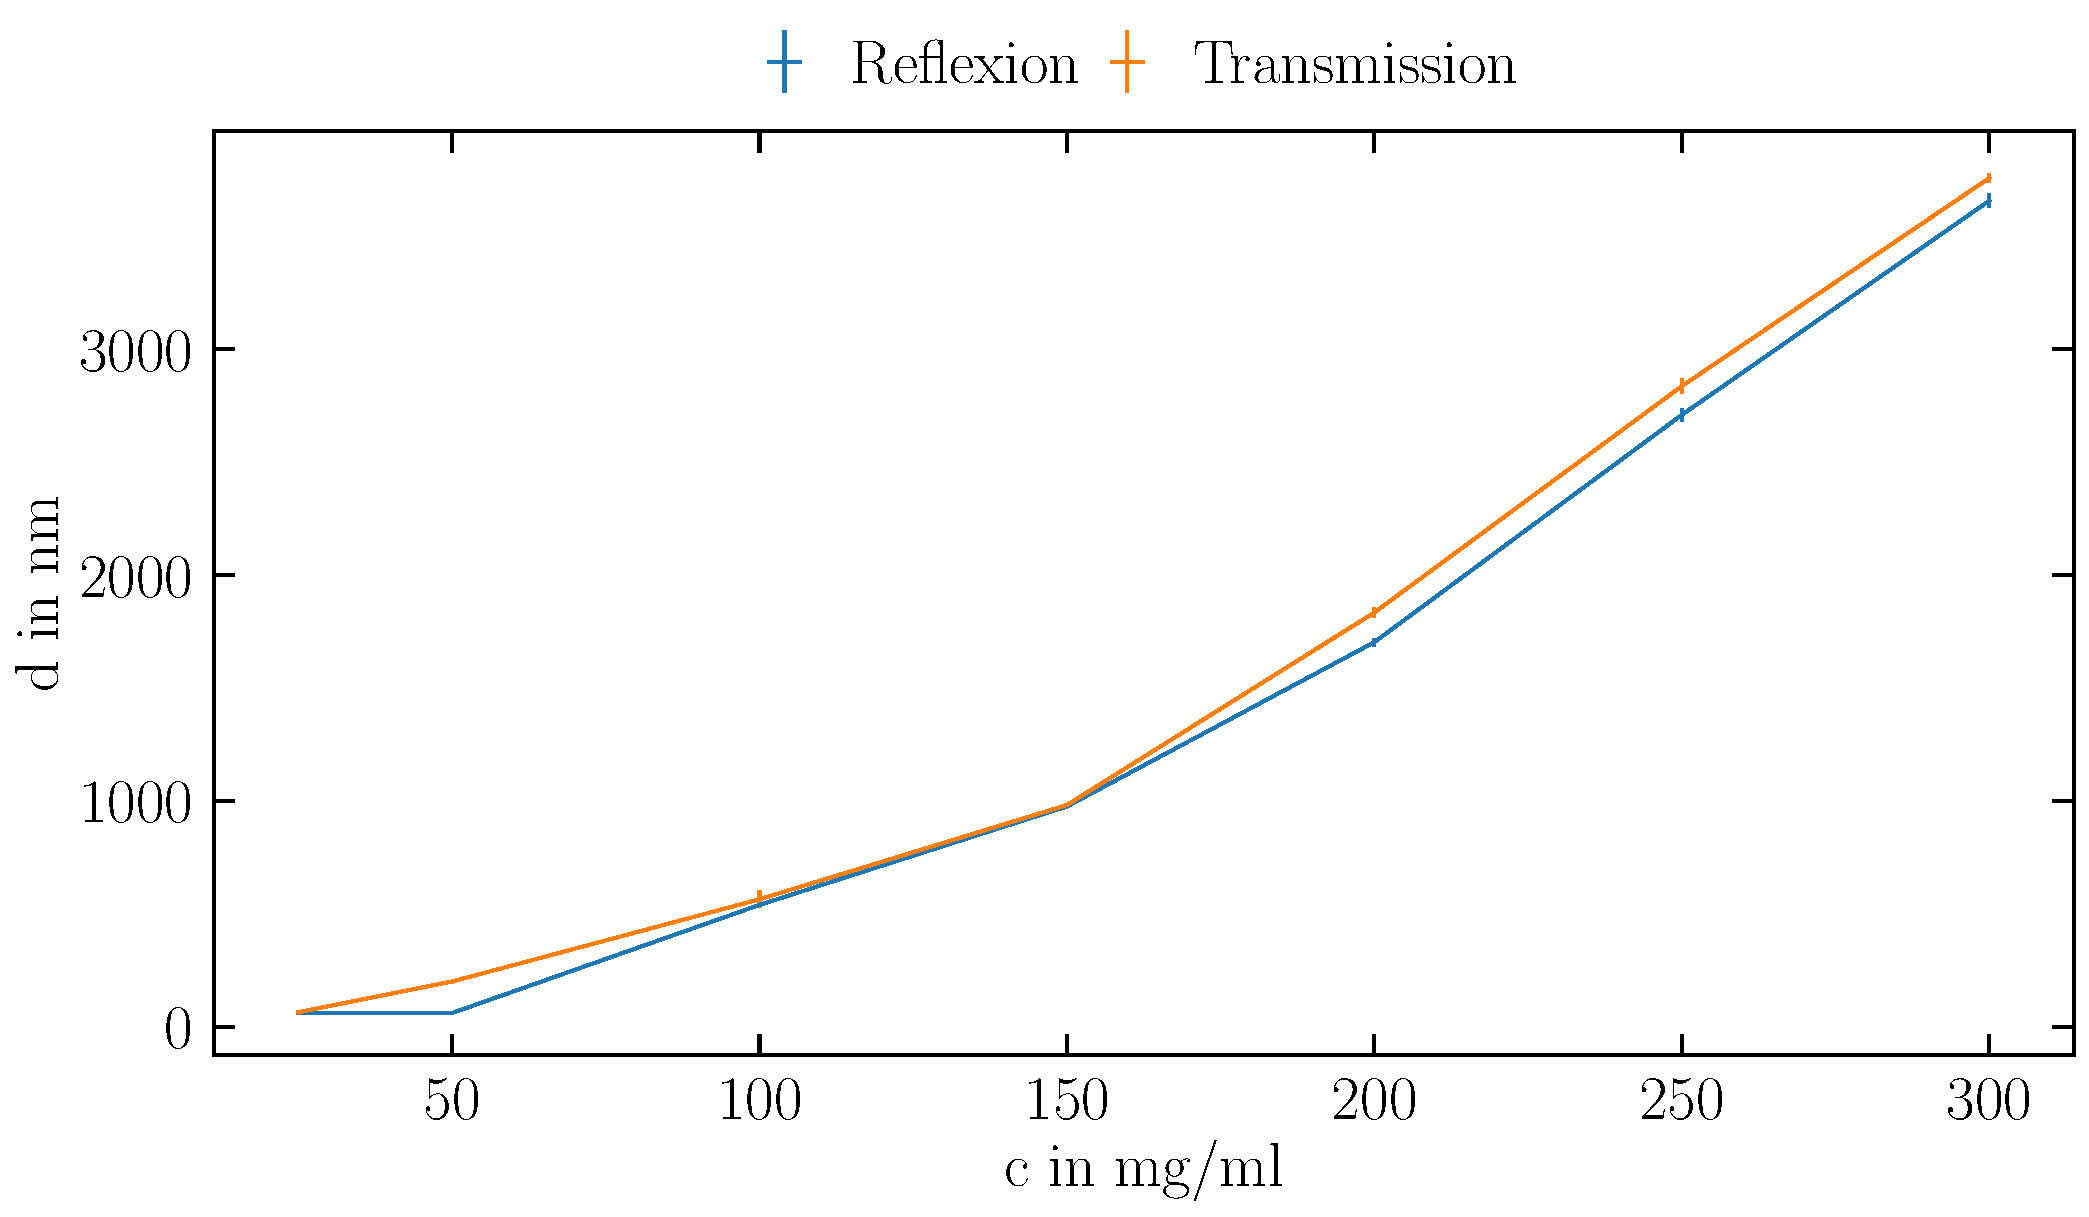
\includegraphics[width=0.92\textwidth]{Auswertung/43/Schichtdicken-Beide.pdf}
	\captionof{figure}{Schichtdicken $d$ der Proben in Abhänigkeit von der Konzentration der Polymerlösung $c$.}
	\label{fig:fitgueteReflexion}
\end{center}

Besoders hervorstechend ist ein Knickpunkt bei etwas über $150$ mg/ml rechts von disem scheint eine lineare Abhängikeit zwischen Konzentration und Schichdicke zu bestehen.

Links von dem Knickpunkt ist auch eine lineare abhänigkeit vorstellbar, jedoch fällt für niedrige Konzenrationen auf, dass mochlicherweise eine asymtotische Annäherung gegen eine Minimaldike stattfindet. Dies wird besonders deutlich wenn die durch Reflexion gewonnenen Messwerte betrachtet werden. Wohingegen eine linearer Abfall bei den Messwerten der Transmission vermutet werden kann. Prinzipiell würde eine Annäherung zu einer Minimaldicke plausibel wirken, da man vermuten könnte, dass sich eine Polymer-Monolage für kleine Konzentrationen ausbildet. Auch die Größenordnung, von um die $60$ nm, dieser kleinsten Dicke setzt dem nichts entgegen.

Abgesehen von den Differenzen bei kleinen Konzentrationen ist noch eine kleine Verschiebung bei großen Konzentrationen zu sehen. Jedoch scheint diese vernachlässigbar zu sein.


\newpage
\subsection{Bestimmung der kritischen Überlapp-Konzentration $c_0$}

Zur Bestimmung der kritischen Überlapp-Konzentration wurde im Bereich vor und nach dem Knick je ein linearer Fit durchgeführt. Somit konnte die Stelle des knicks und die kritischen Überlapp-Konzentration genau bestimmt werden.

Verwendete Fitfunktion:
\begin{gather}
	y = ax + b
	%\caption[]{Lineare Fitfunktion}
\end{gather}

Fit:
\begin{center}
	\captionsetup{type=figure}
	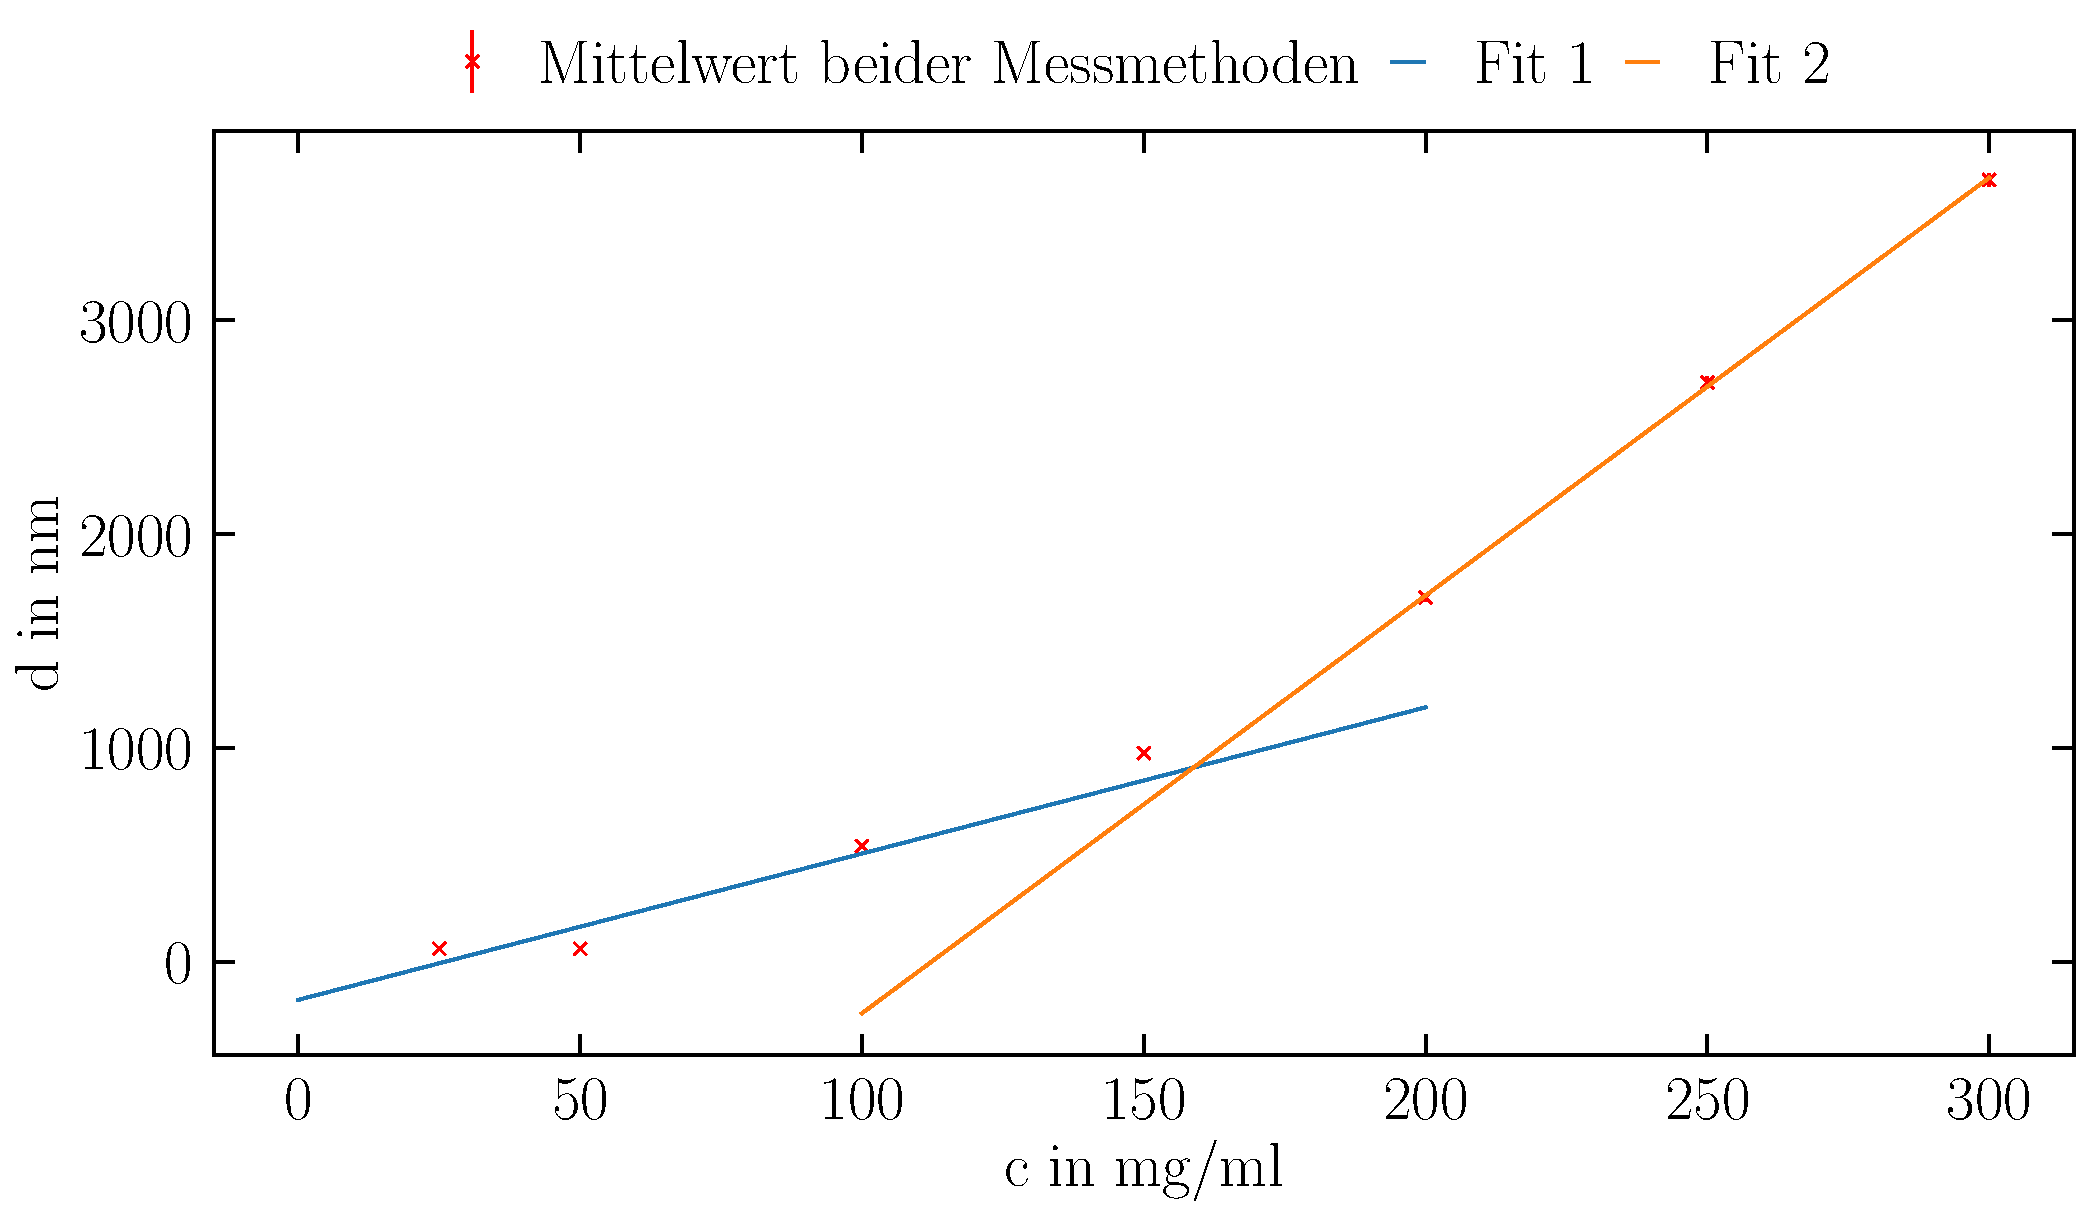
\includegraphics[width=0.92\textwidth]{Auswertung/43/Schichtdicken-Fit.pdf}
	\captionof{figure}{Mittelwert der Schichtdicken $d$ der Proben, aus beiden Messwerten, in Abhänigkeit von der Konzentration der Polymerlösung $c$. Und lineare Fits zur ermittelung der kritischen Überlapp-Konzentration $c_0$.}
	\label{fig:fitgueteReflexion}
\end{center}

\begin{table}[h]
	\centering
	\begin{tabular}{r|c|c}
		& a & b \\ \hline
		Fit 1 & 6,84 & -178,86 \\
		Fit 2 & 19,54 & -2195,79
	\end{tabular}
	\caption[]{Ergebnisse des linearen Fits.}
\end{table}

Da $c_0$ die x-Koordinate des Schnittpunktes ist, kann die volgendermaßen berechnet werden:
\begin{align}
	c_0 &= \frac{b_2 - b_1}{a_1 - a_2}\\
	\Rightarrow c_0 &= (159 \pm 1) \, \frac{\text{mg}}{\text{ml}}
\end{align}

\subsection{Berechnung der root-mean-square end-to-end distance}

\paragraph*{Nach Mark}
Die root-mean-square end-to-end distance wird im folgenden, ausgehend vom charakteristischen Flory Verhältnis von $C_\infty = 9.5$ berechnet. Heirzu wird folgende Formel benutzt:
\begin{gather}
	R_{rms} = \sqrt{C_\infty n l^2}
\end{gather}
Wobei $l$ die Länge im Polymerrückrat ist (Annahme: $l = 1.54$ Anström) und n die Anzahl der Bindungen im Polymerrückrat ist. (??)

\paragraph*{Nach Daum}
Nun wird root-mean-square end-to-end distance mittels folgender Formel berechnet:
\begin{gather}
	R_{rms} = 2,84 \cdot 10^{-8} \cdot \sqrt[3]{\frac{M}{c_0}}
\end{gather}
Wobei $M$ das Molekulargewicht des Polymers ist und $c_0$ die kritische Überlapp-Konzentration.

\newpage
\subsection{Vergleich der Messdaten mit den bekannten Polymer Modellen}

Die Gleichungen der Überlapp-Konzenrationen für Übergang von verdünnt zu semiverdünnt $C^*$ und semiverdünnt zu konzentriert $C^{**}$ wurden aus dem Paper "Overlap Concentration of Macromolecules in Solution"von Qicong Ying und Benjamin Chu aus 1987 entnommen.

Wobei bei den Formeln aus dem Paper M die molekulare Masse des Polymers, $N_A$ die Avogadrokonstante, $h_0$ die root-mean-square end-to-end distance, $\rho$ die Persistenzlänge und L die Konturlänge, d der Konturdurchmesser und $[\eta]^{**}$ die intrinsische Viskosität ist.

\begin{figure}[h]
	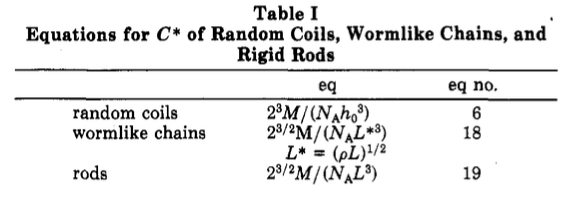
\includegraphics[width=0.95\textwidth]{Bilder/Auswertung/43/YingT1.png}
	\caption[short]{Gleichungen für $C^*$ aus Ying et al. (1987).}
\end{figure}


\begin{figure}[h]
	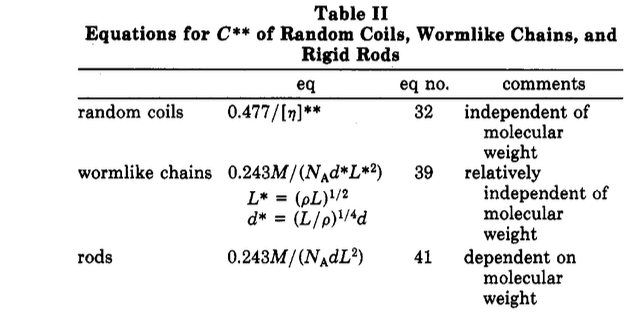
\includegraphics[width=0.95\textwidth]{Bilder/Auswertung/43/YingT2.png}
	\caption[short]{Gleichungen für $C^{**}$ aus Ying et al. (1987).}
\end{figure}

% etc.

    % 5.Kapitel Fazit
    % 5. Einleitung

\chapter{Fazit}
\label{chap:fazit}

Abschließend lässt sich sagen, dass durch ausführung des Versuches ein tieferes Verstäntnis für hochauflösende Molekülspektroskopei gewonnen wurde. Auserdem wurden Erfahrungen im Umgang mit Lock-In-Verstärker und HF Leitungen gesammelt, welche bis dato selten benutzt worden sind. Auch der Umgang mit der dB bzw. dBm Skala konnte geübt werden. 

    % Anhang
    % Anhang

\appendix

% Text

% Appendix A

\chapter{Append A}
\label{chap:AppendA}

\section{Append A}


    % Literatur
    \bibliographystyle{Auswertung.bst}
    \nocite{*}
    \bibliography{Auswertung.bib}

\end{document}
